% !TeX root = ../../main.tex

% \subsection{Simplicial Complexes}\label{sec:complexes}

\begin{figure}[htbp]
  \centering
  % 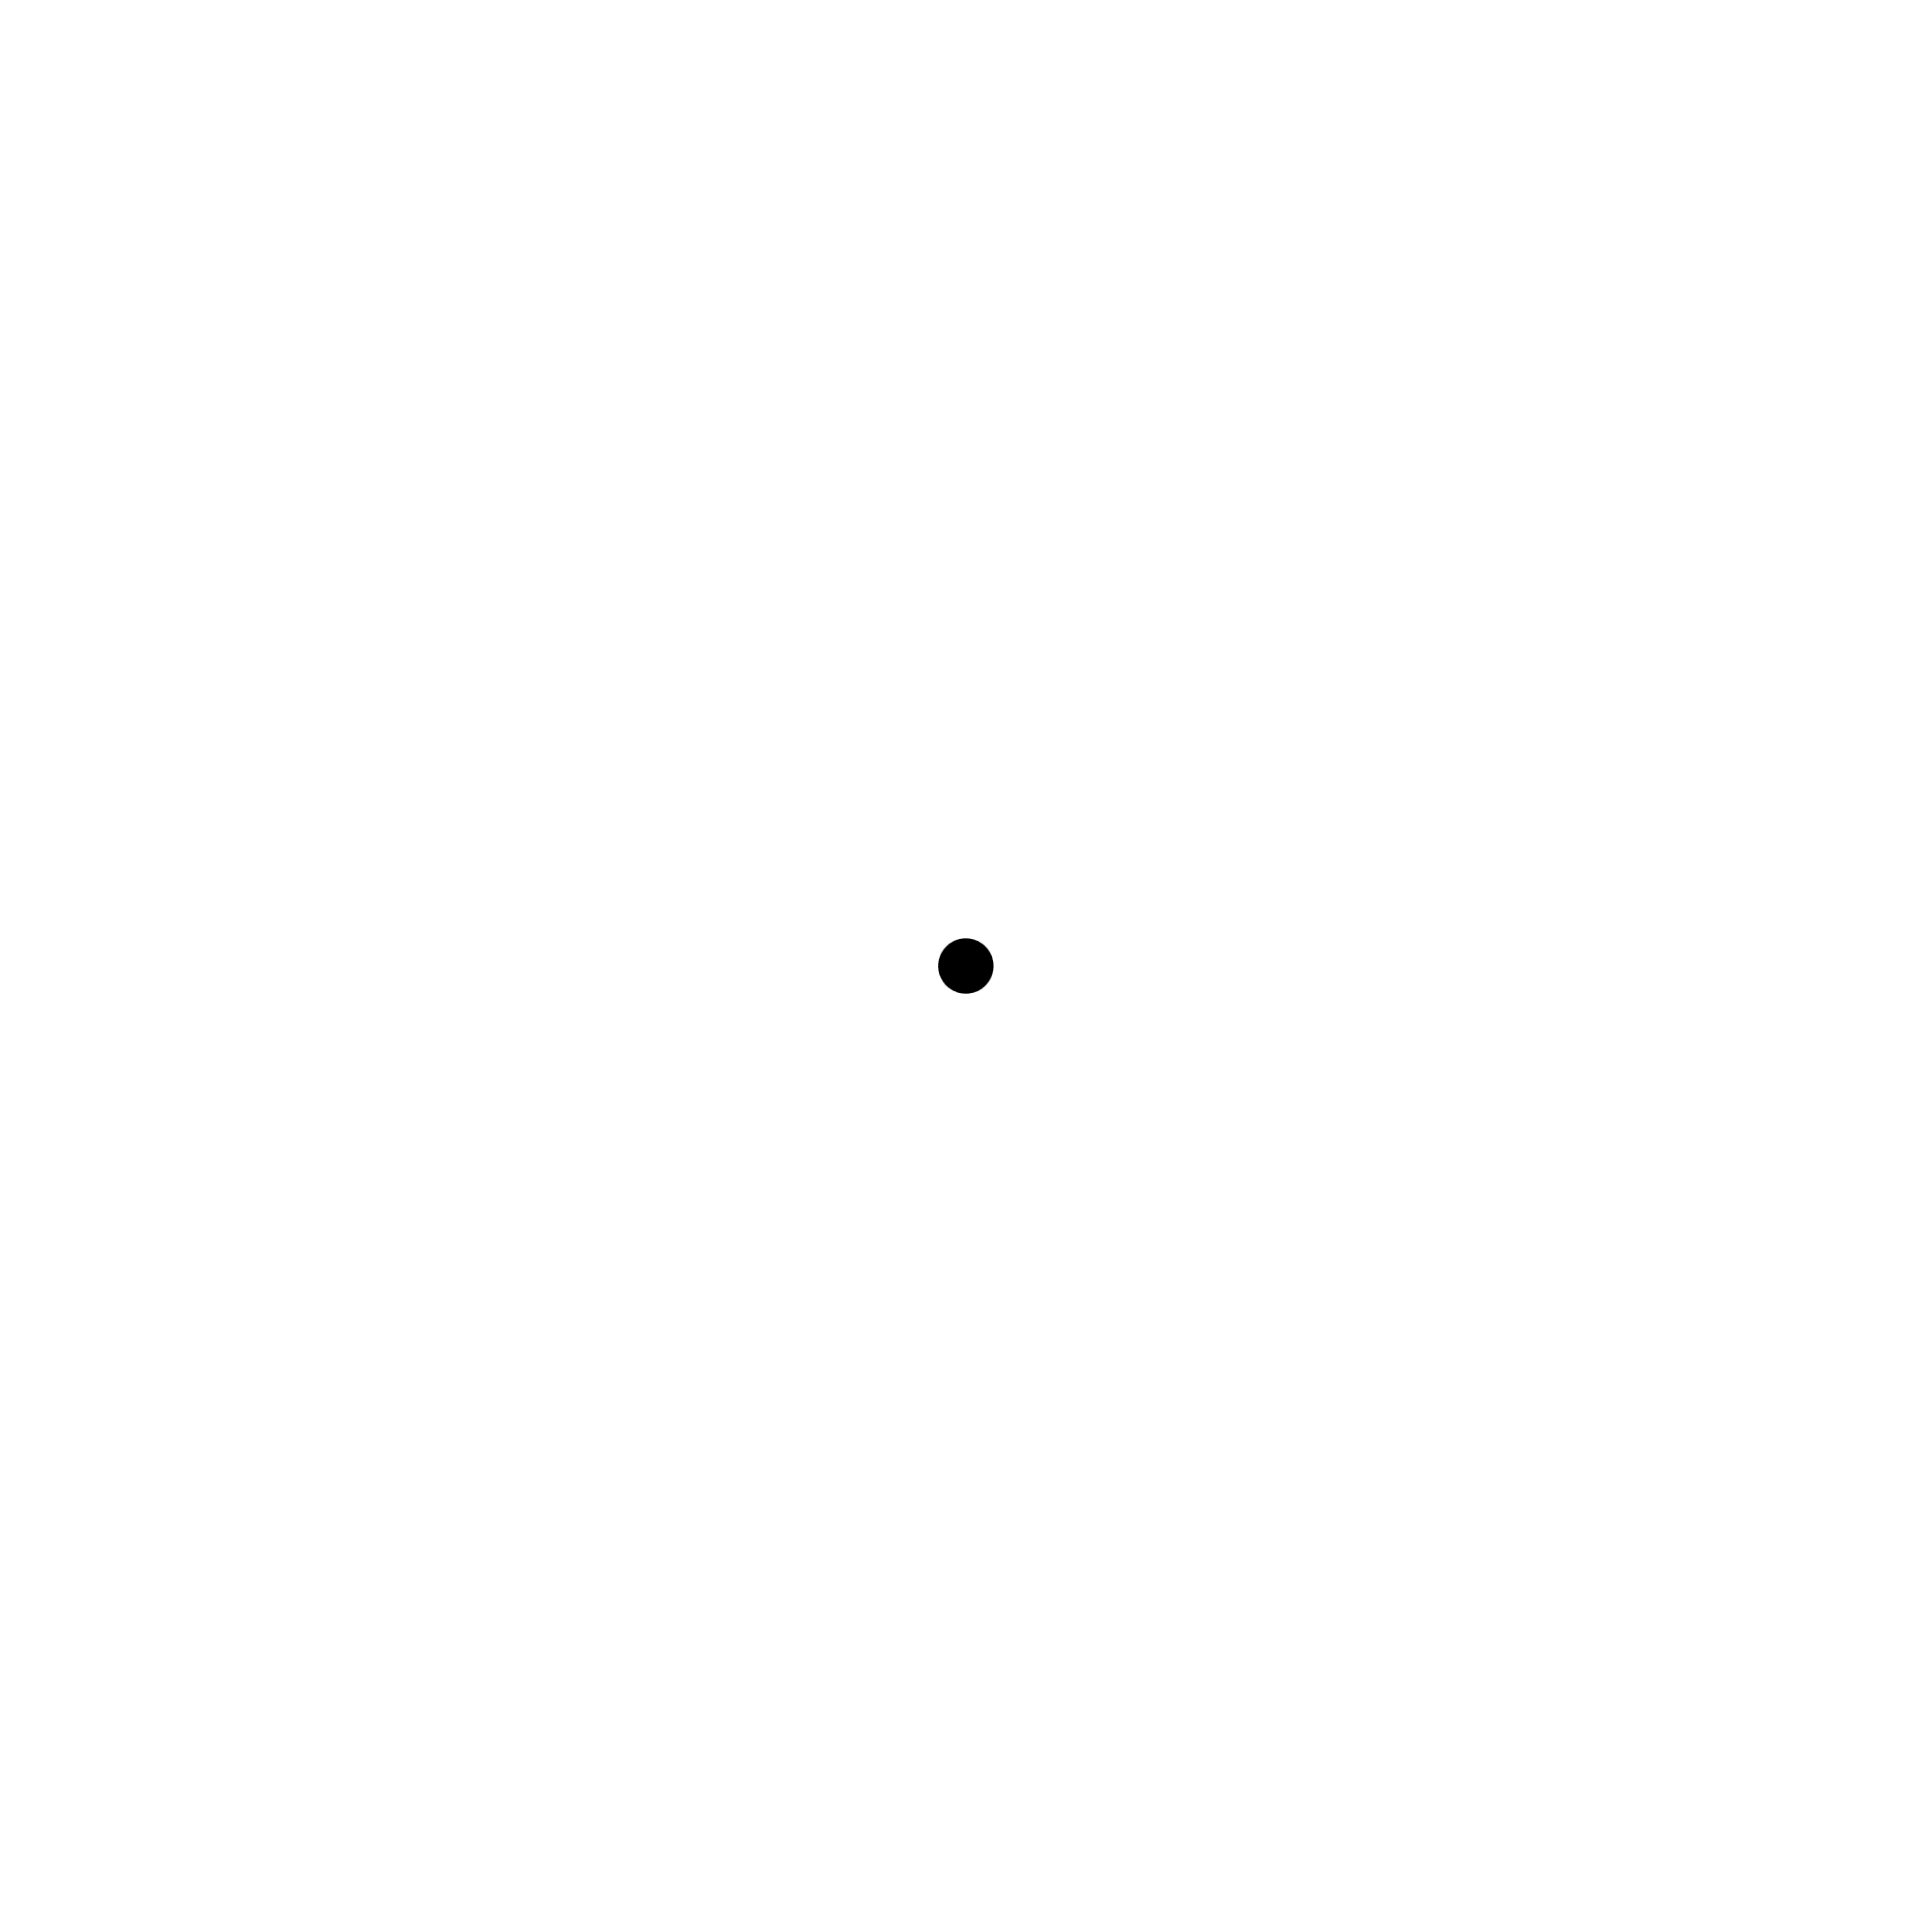
\includegraphics[width=0.2\textwidth]{figures/component.png}
  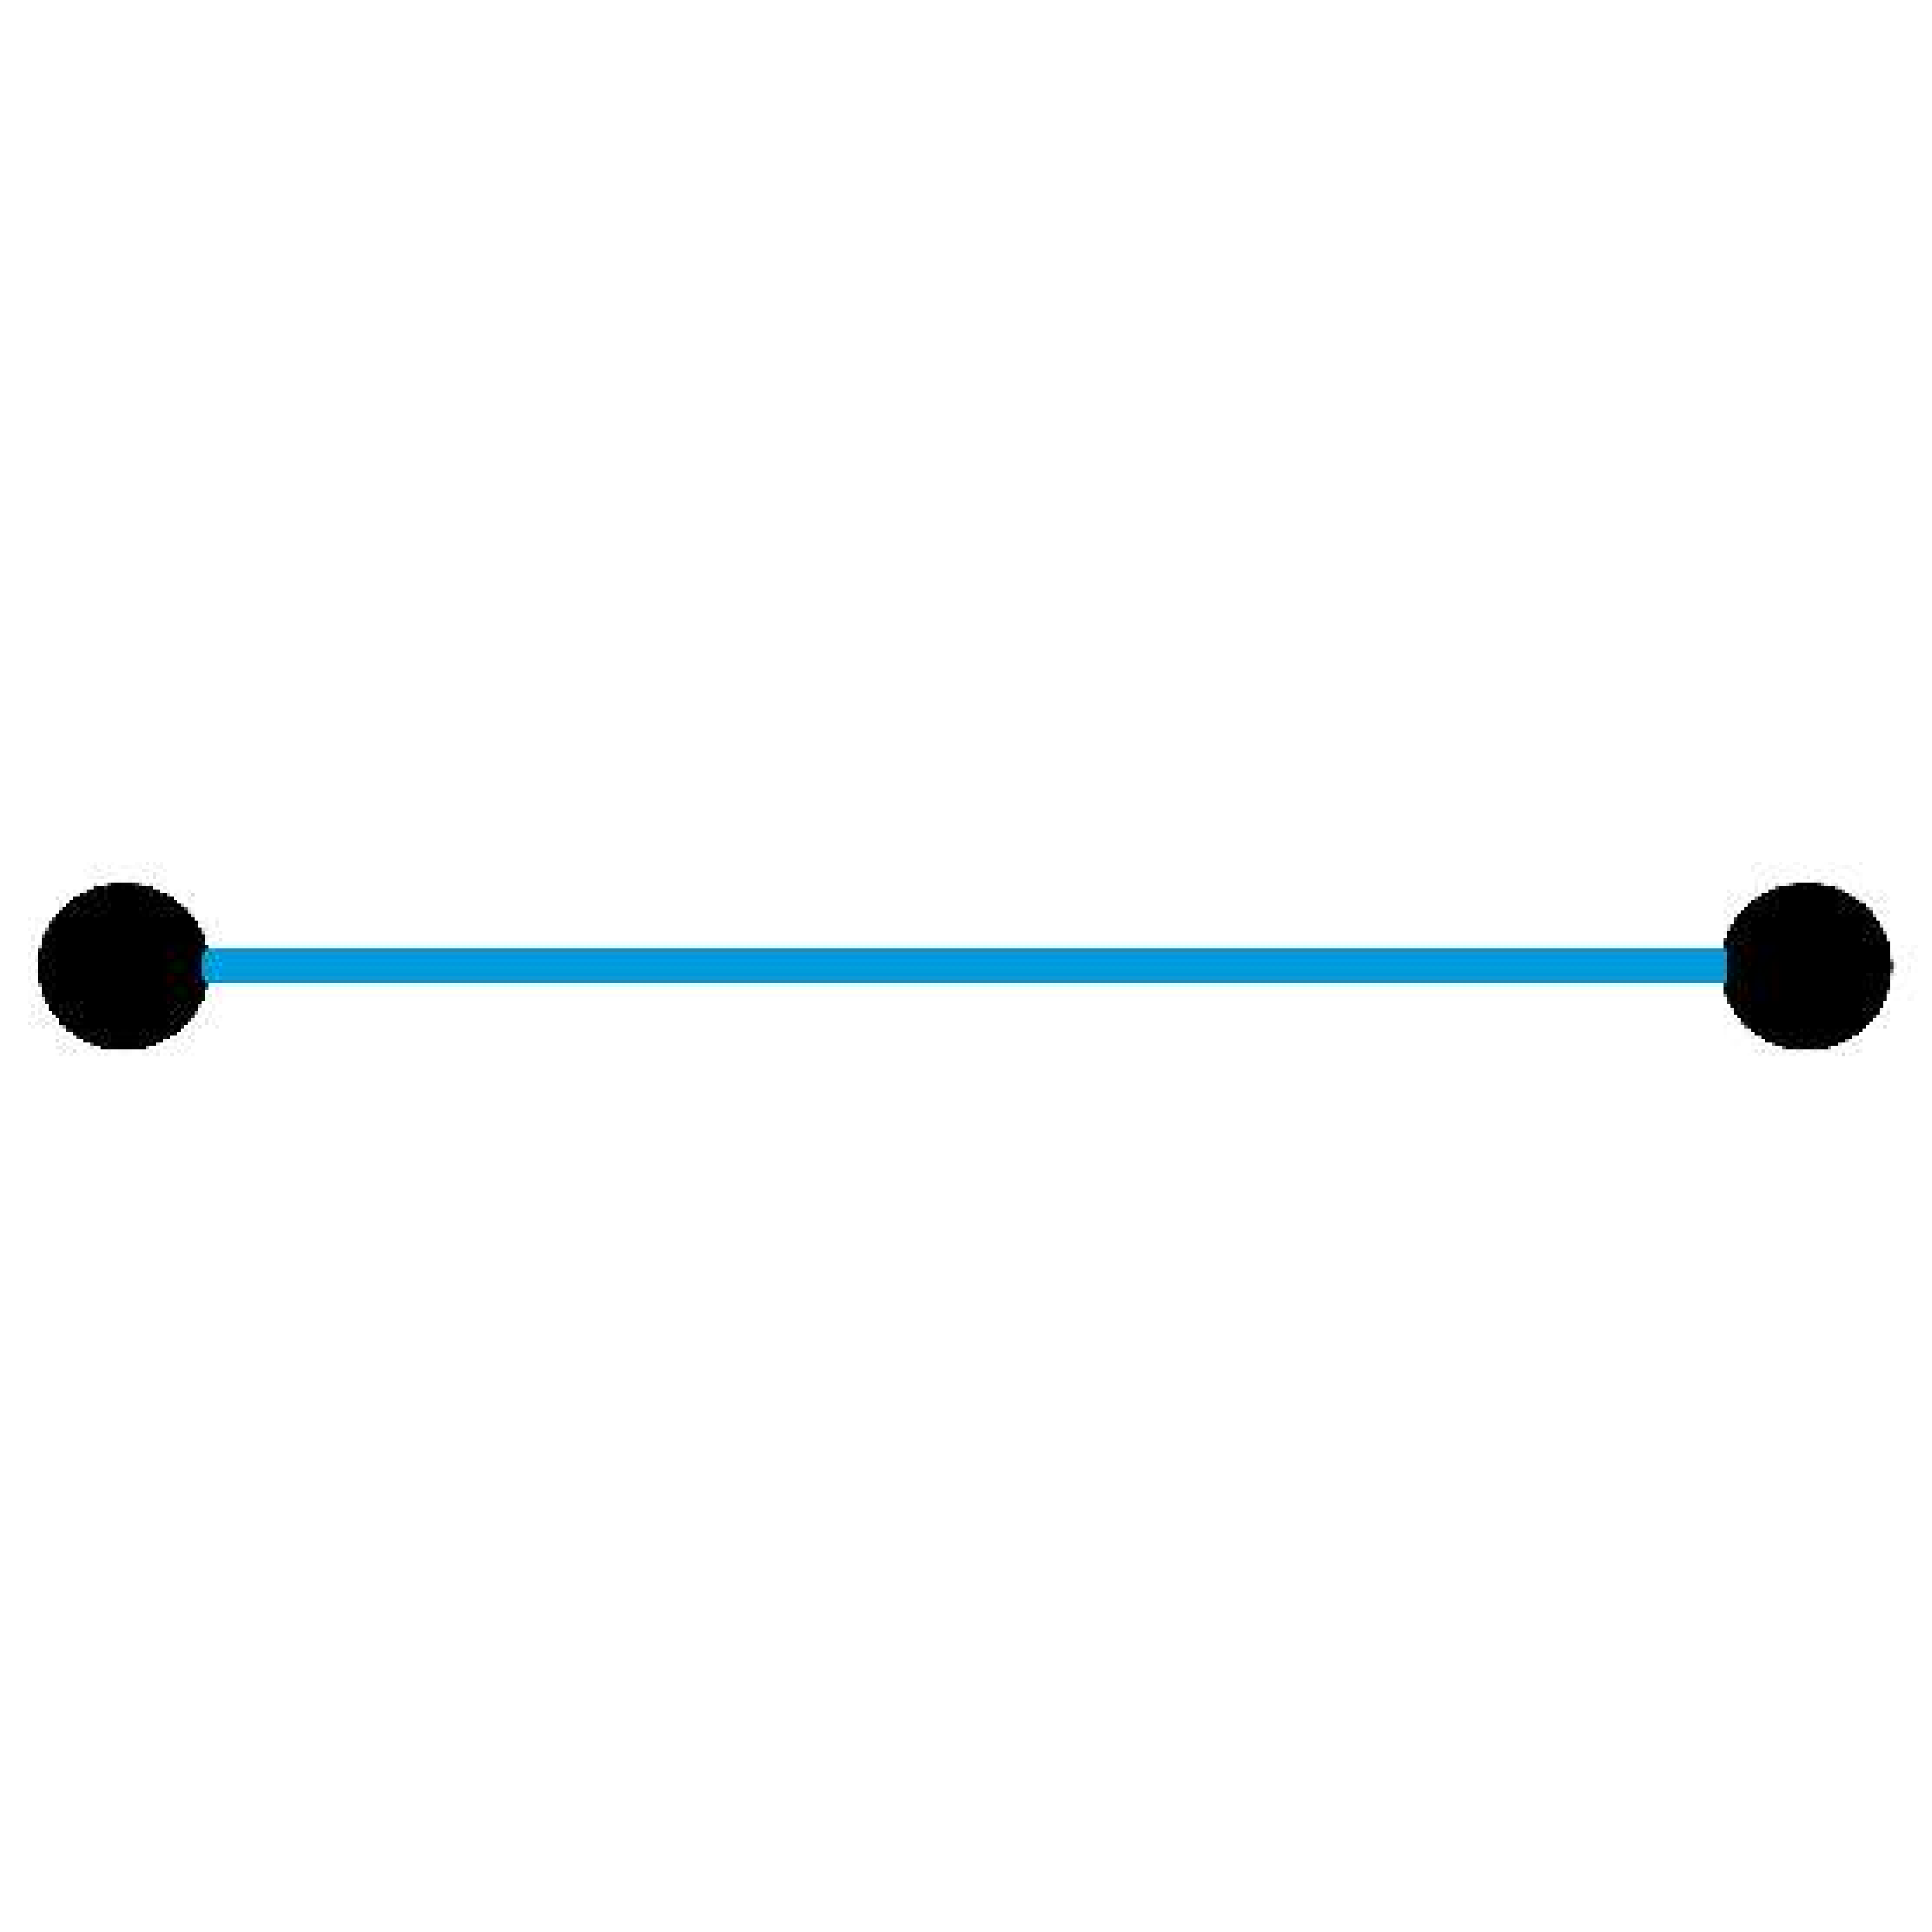
\includegraphics[width=0.2\textwidth]{figures/edge-comp.pdf}\hspace{3ex}
  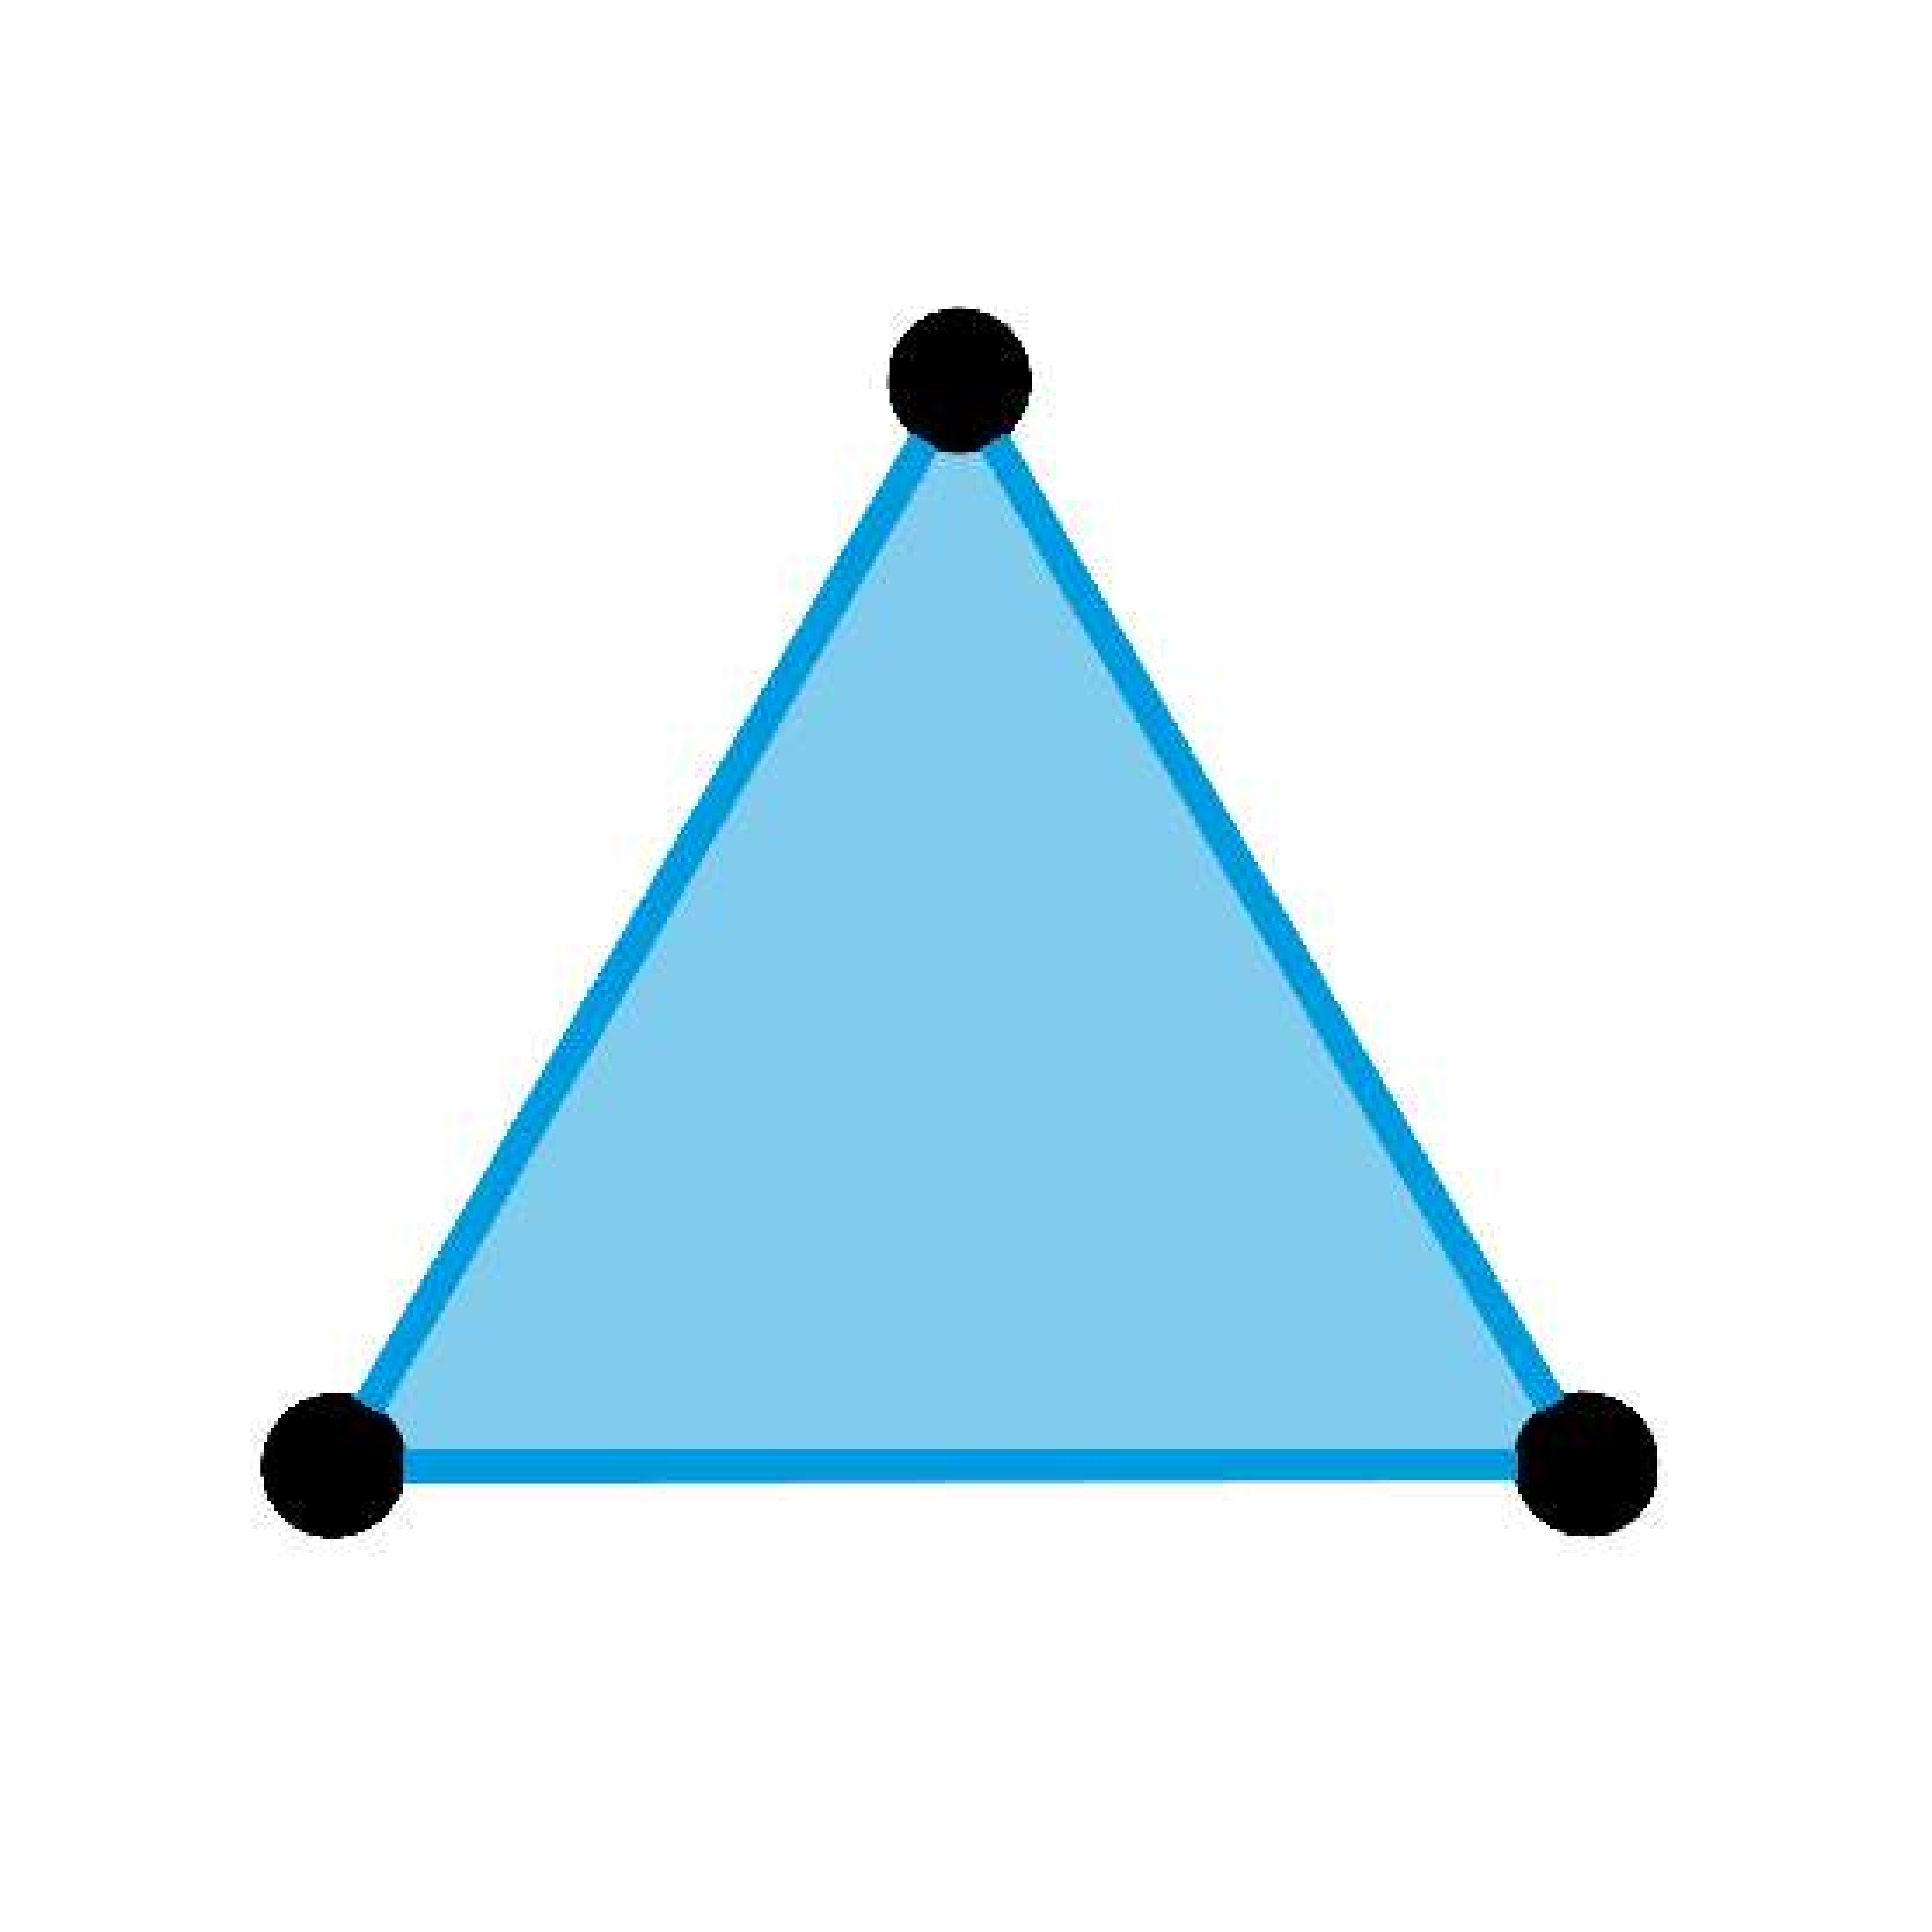
\includegraphics[width=0.2\textwidth]{figures/tri-comp.pdf}\hspace{3ex}
  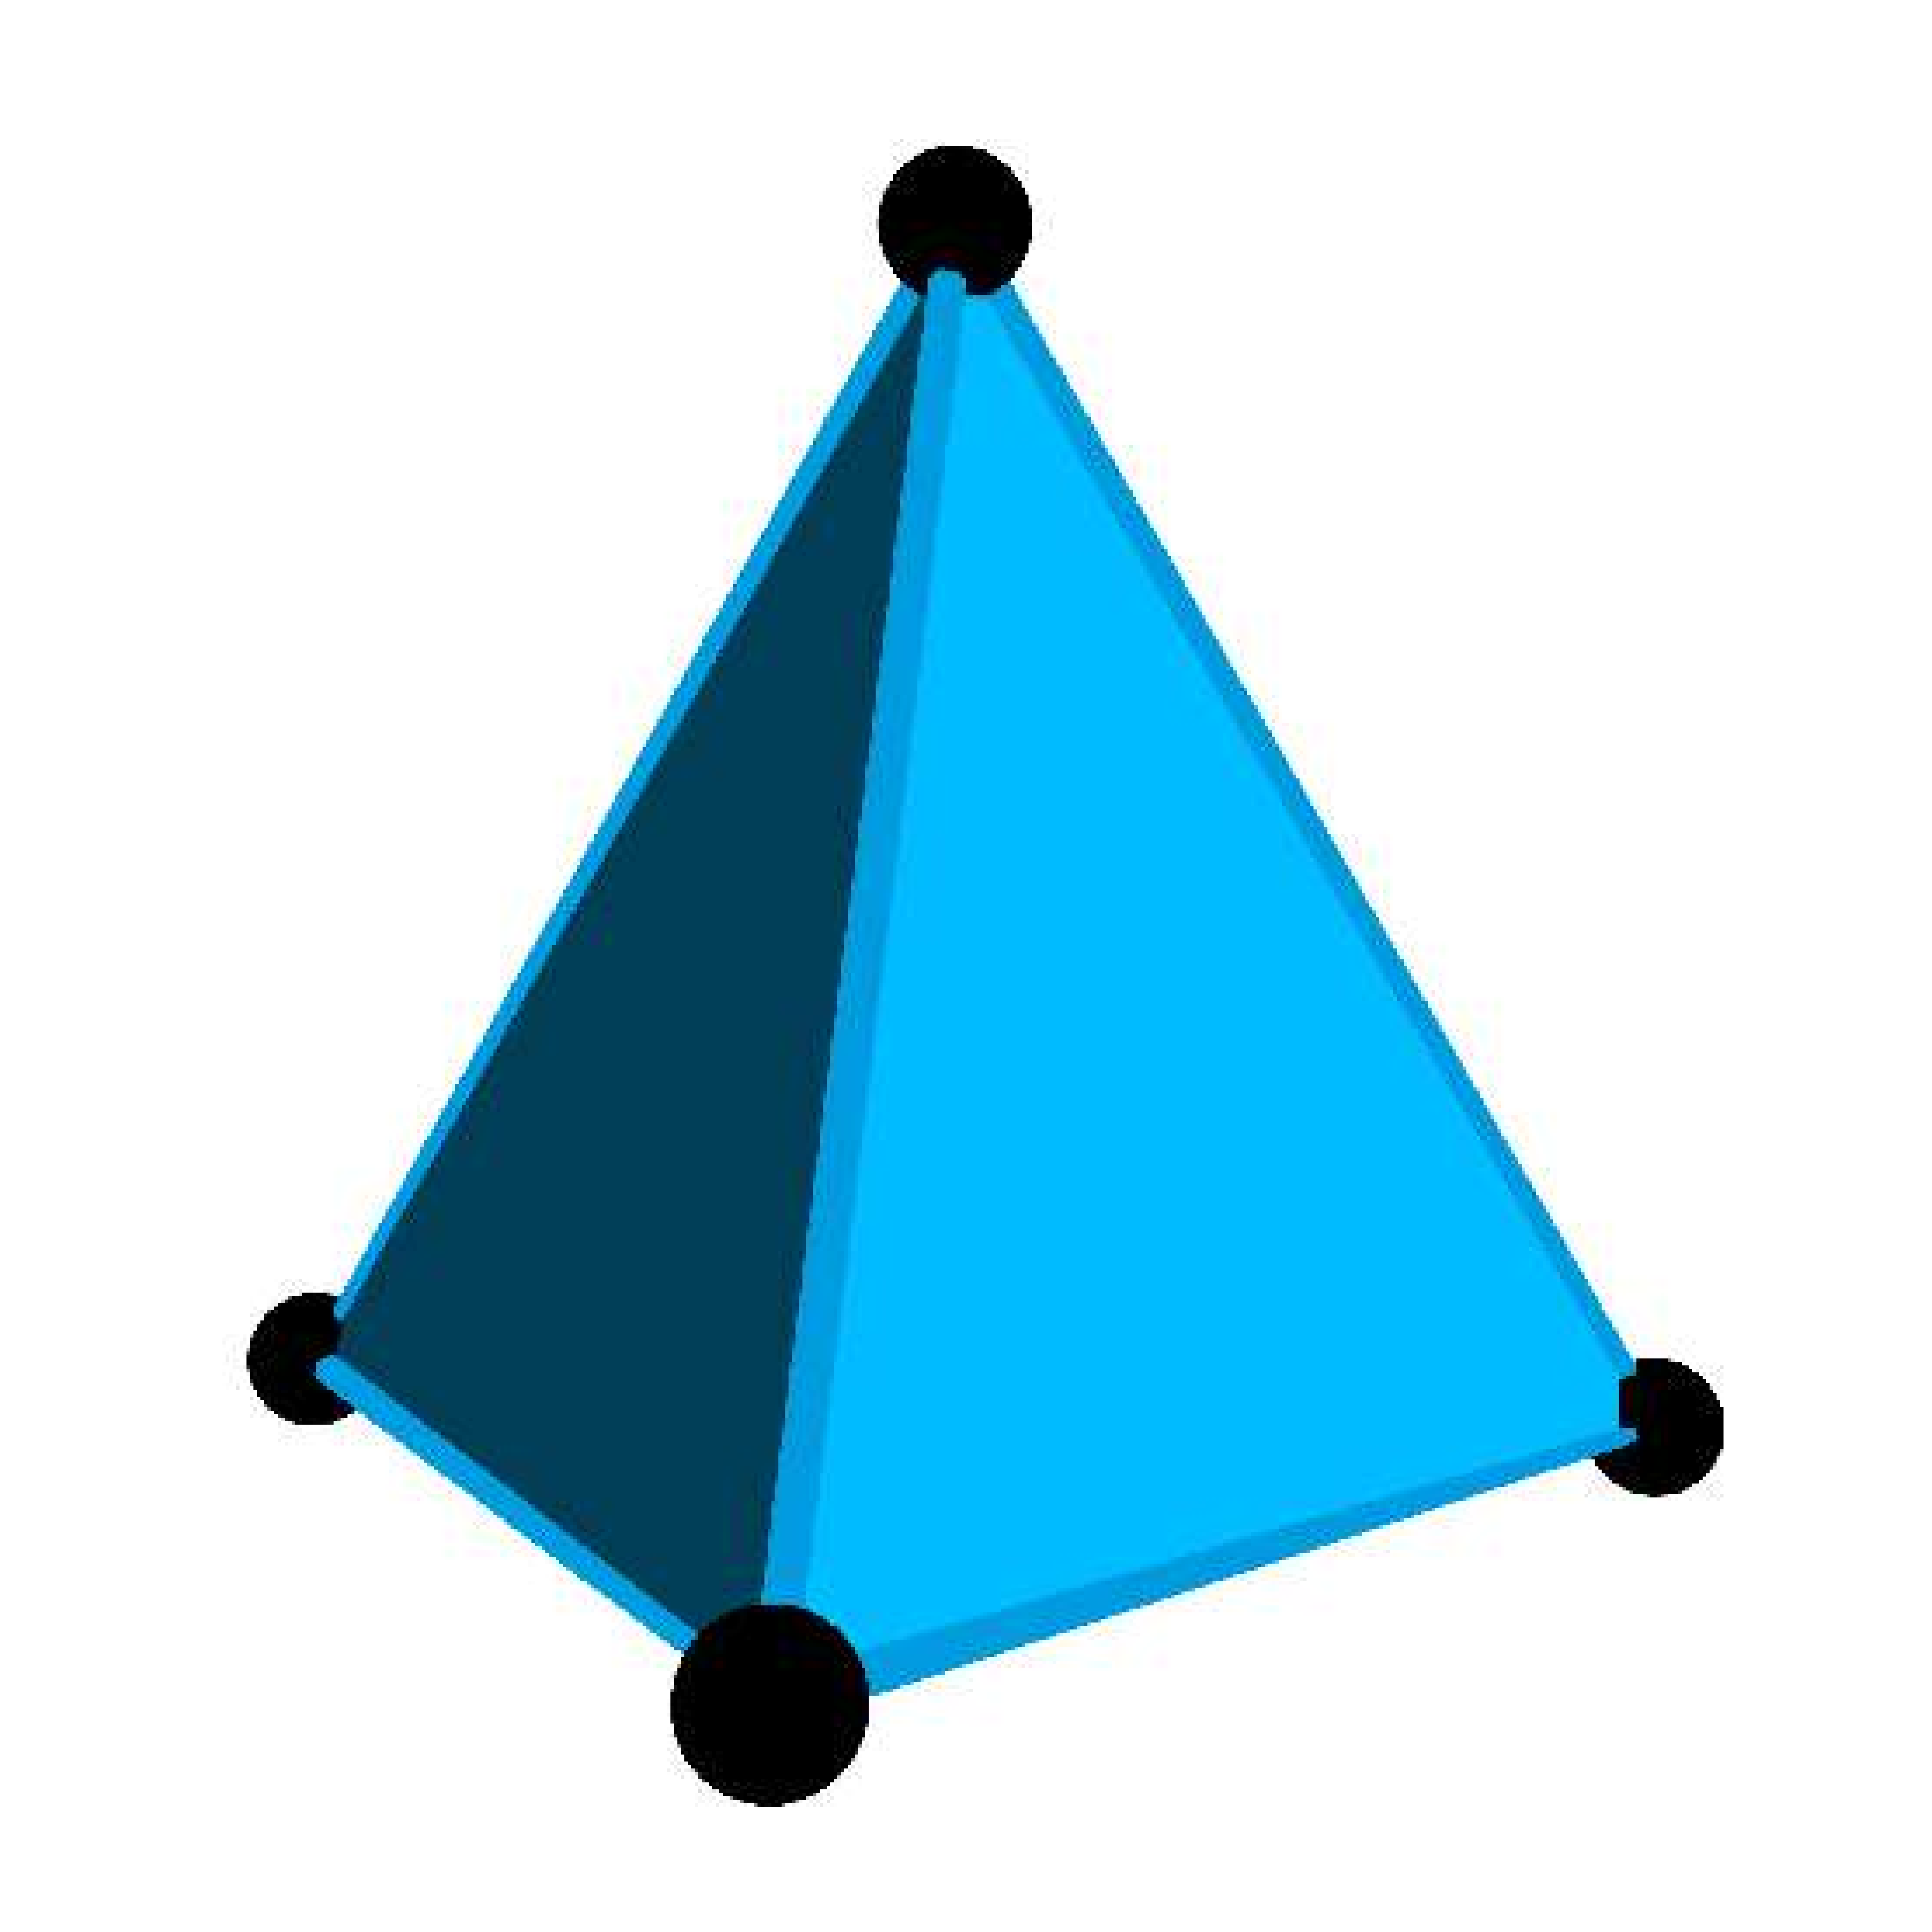
\includegraphics[width=0.2\textwidth]{figures/tet-comp.pdf}
  \caption{Simplices of dimension 1-3.}\label{fig:simplices}
\end{figure}

A \textbf{simplicial complex} $K$ is a collection of subsets, called \textbf{simplices}, of a vertex set $V$ such that for all $\sigma\in K$ and $\tau\subset\sigma$ it must follow that $\tau\in K$.
The \textbf{dimension} of a simplex $\sigma\in K$ is defined as $\dim(\sigma) := |\sigma|-1$ where $|\cdot|$ denotes set cardinality.
The dimension of a simplicial complex $K$ is the maximum dimension of any simplex in $K$.
That is, a graph is a 1-dimensional simplicial complex in which vertices and edges are 0 and 1-dimensional simplices, respectively.

% \figblock{%
% \begin{figure}[htbp]
% \centering
%     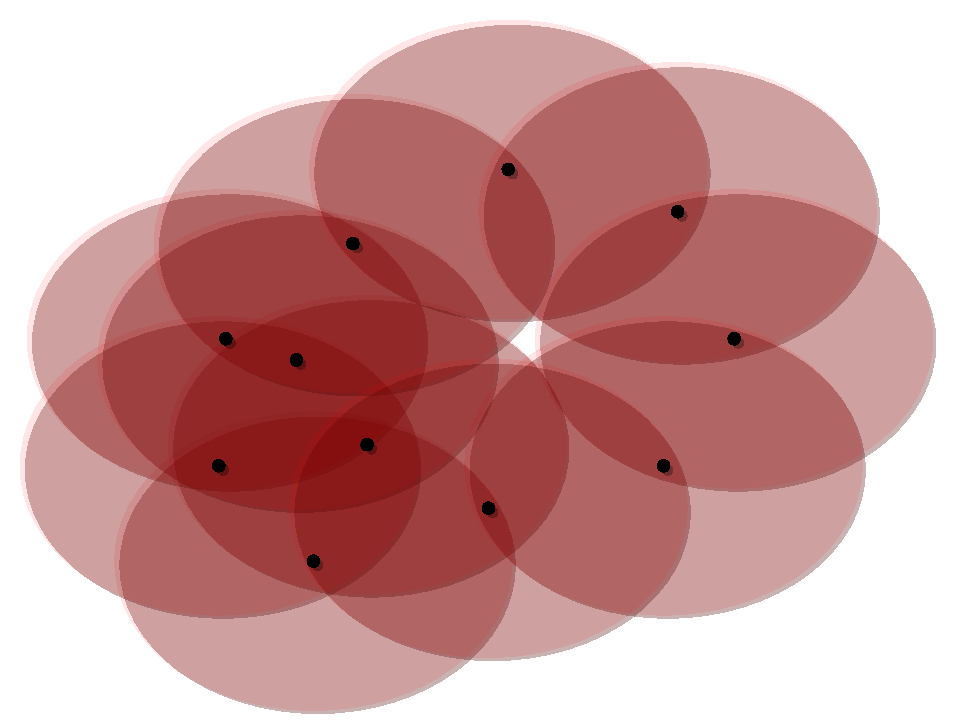
\includegraphics[scale=0.33]{figures/holes_cover.pdf}
%     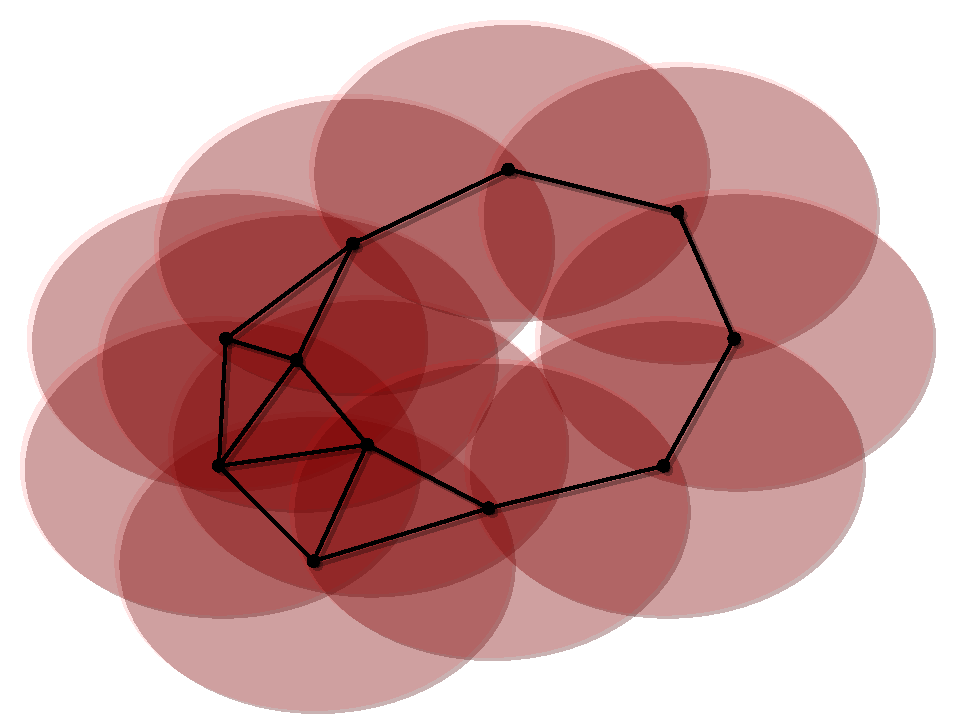
\includegraphics[scale=0.33]{figures/holes_edges.pdf}
%     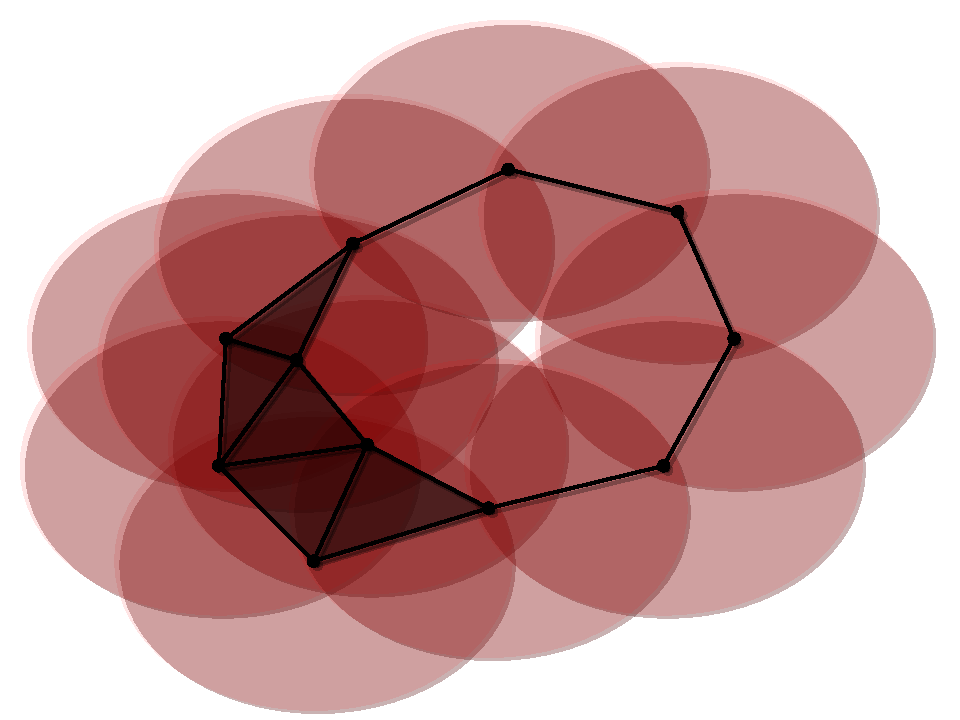
\includegraphics[scale=0.33]{figures/holes_complex.pdf}
%      \caption{(Left) The coverage regions of a collection of points $P$ at some scale $\alpha$.
%             (Middle) The neighborhood graph with edges for each pair of points within pairwise distance $\alpha$.
%             (Right) If we attempt to fill cycles in the graph with triangles identify a cycle that cannot be filled which reflects a gap in coverage}
%      \label{fig:holes}
% \end{figure}}

It is natural to think of a $k$-dimensional simplicial complex as the generalization of an undirected graph consisting of vertices and edges, collections of at most 2 vertices, to collections of sets of at most $k+1$ vertices.
% Just as we have defined a hole in our graph $G$ as a cycle that cannot be filled with triangles, we define a $k$-dimensinal hole in a simplicial complex as a $k$-cycle that cannot be filled with $(k+1)$-simplices.
% In the next section we will formally define $k$-cycles and introduce simplicial homology as a tool for identifying when and which cycles cannot be filled.

\paragraph{Nerves}

% \begin{figure}[htbp]
%   \centering
%   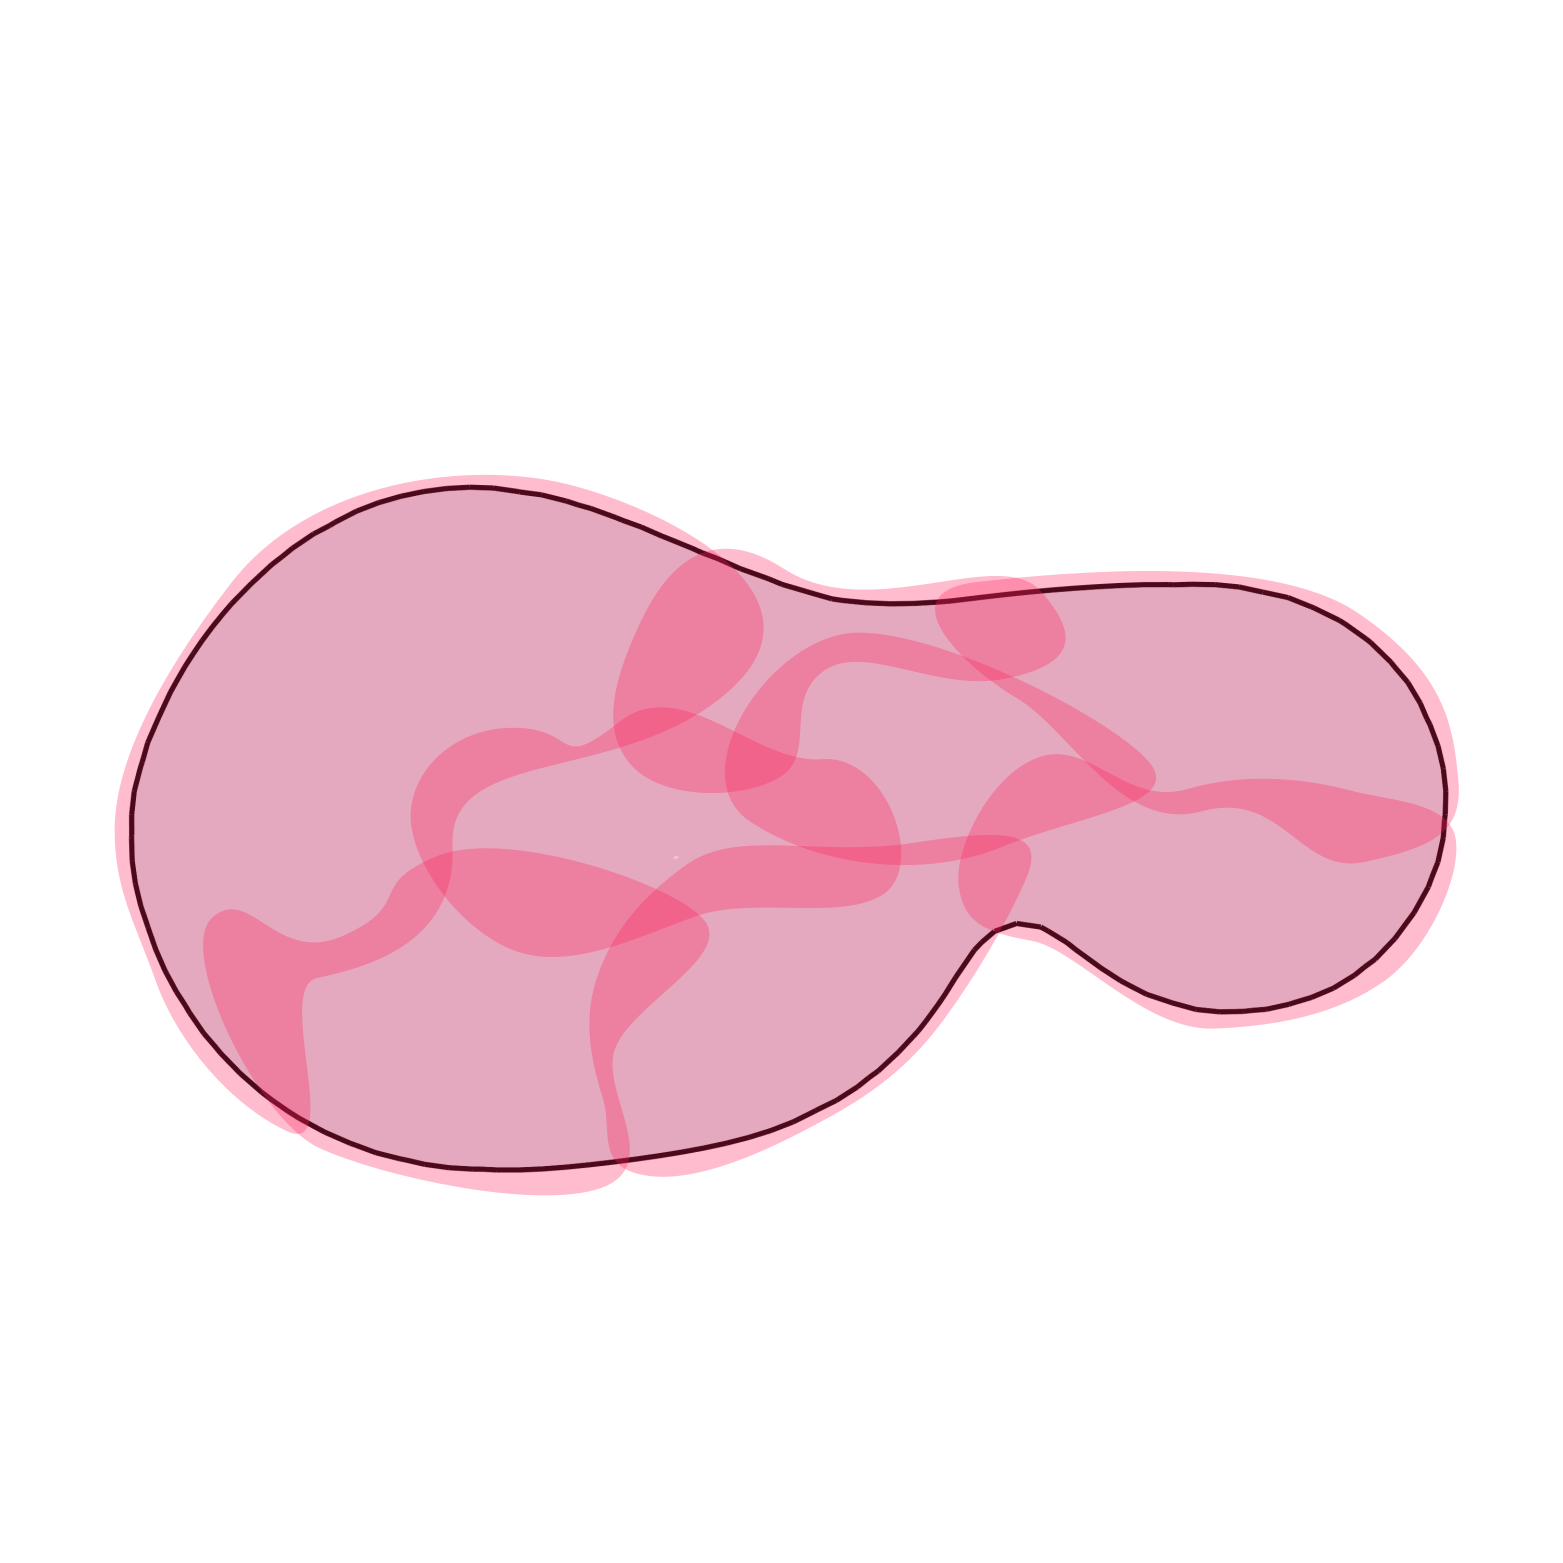
\includegraphics[trim=0 300 0 500, clip, width=0.4\textwidth]{figures/nerves/cover}
%   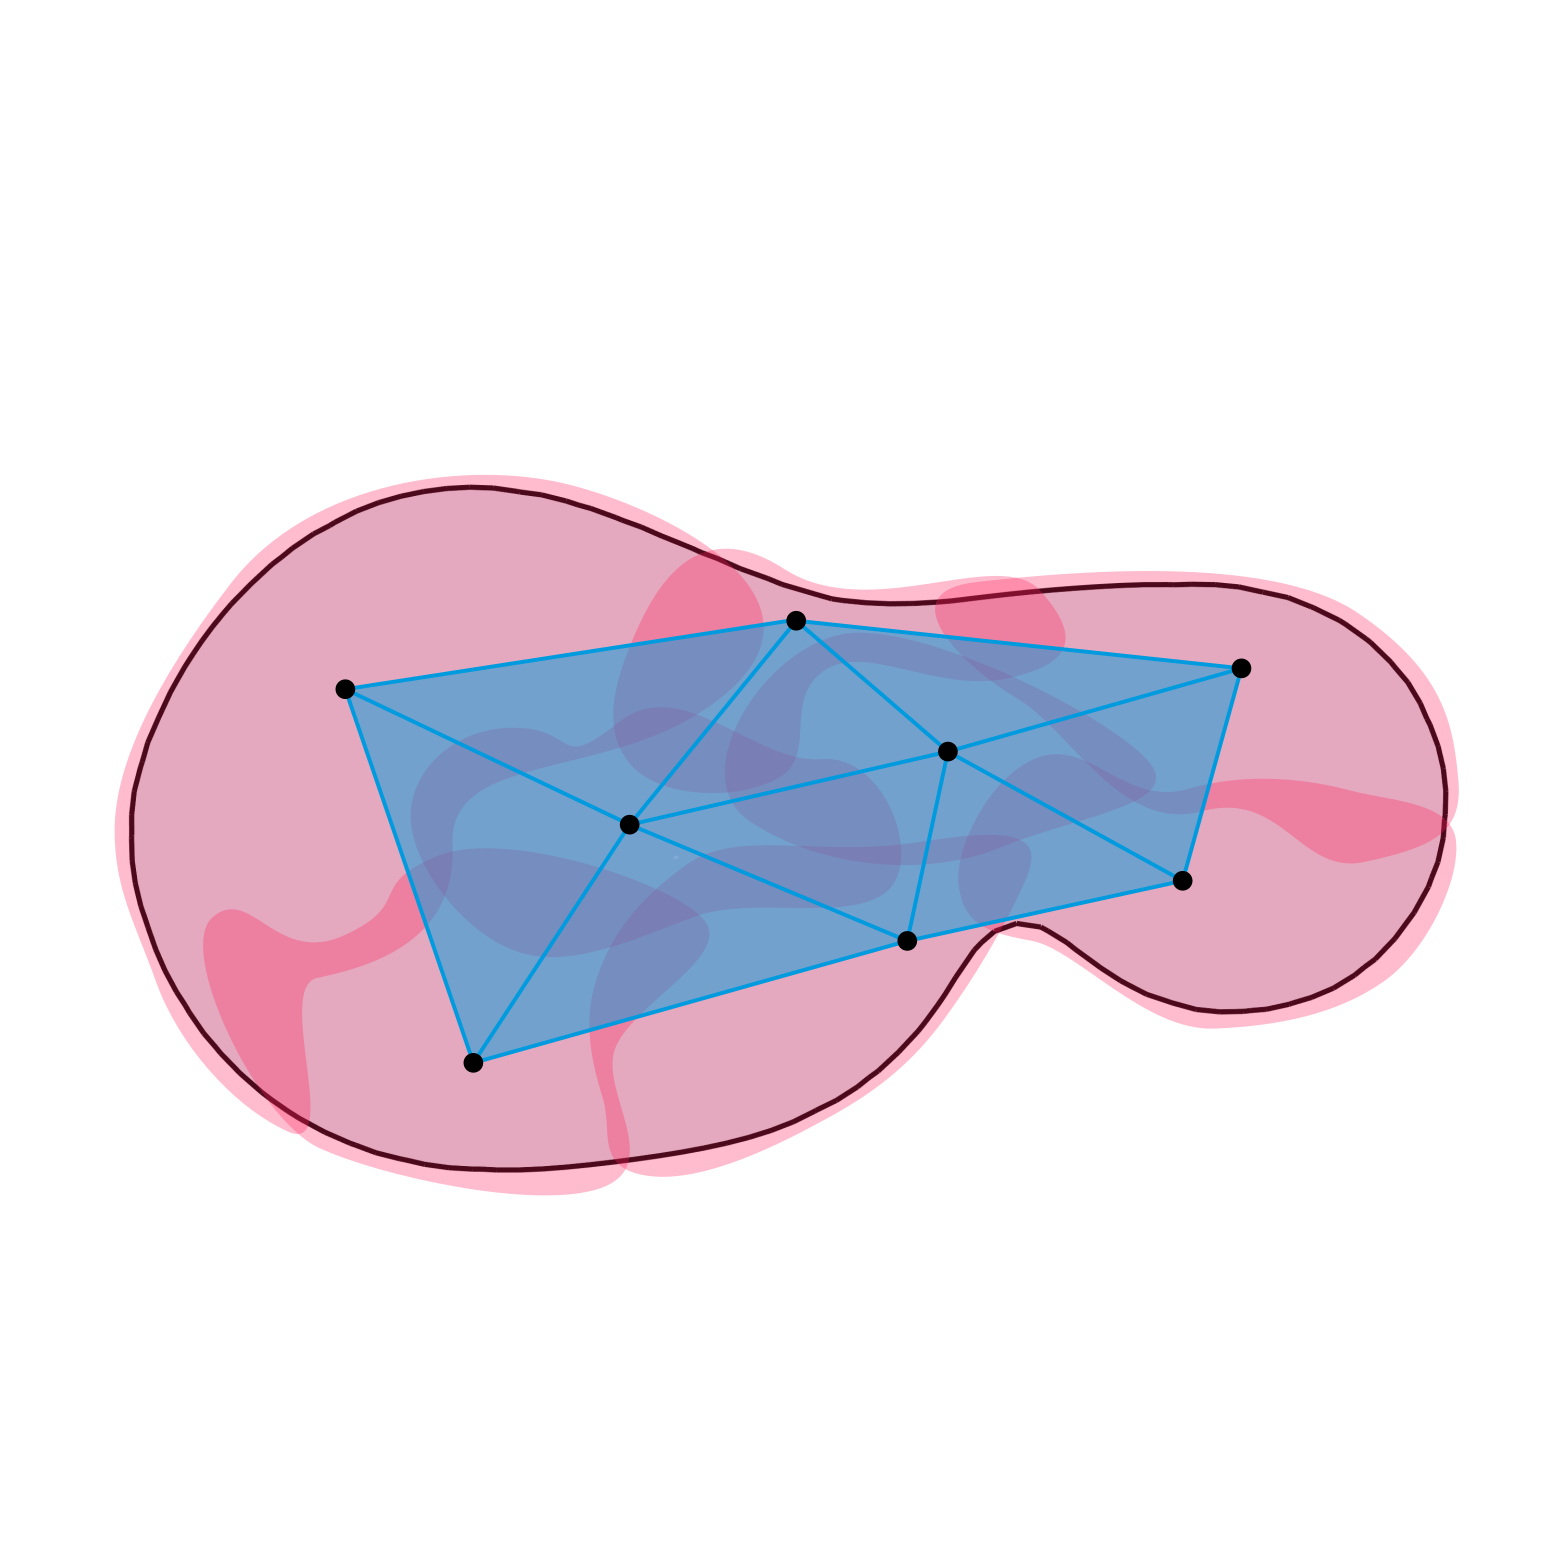
\includegraphics[trim=0 300 0 500, clip, width=0.4\textwidth]{figures/nerves/full}
%   \caption{A cover and its nerve.}\label{fig:nerves}
% \end{figure}

Let $X$ be a topological space.
For some index set $I$ and $U_i\subseteq X$ a collection $\U = \{U_i\}_{i\in I}$ is called a \textbf{cover} of $X$ if $\bigcup_{i\in I} U_i = X$.
The cover is said to be open if all of the sets $U_i$ are open in $X$.
A finite open cover $\U$ is a \textbf{good open cover} if every nonempty intersection of sets in $\U$ is contractible.

There is a simplicial complex associated with any cover $\U$ known as its \textbf{Nerve}, denoted $\N(\U)$, that is defined to be the abstract simplicial complex with vertex set $I$ and simplices $\sigma\subseteq I$ whenever $\bigcap_{i\in\sigma} U_i\neq \emptyset$.
The \textbf{Nerve Theorem} states that whenever $\U$ is a good open cover of a paracompact space $X$ then its nerve $\N(\U)$ is homotopy equivalent to $X = \bigcup_{i\in I} U_i$.
The following is an important result by Chazal et. al.~\cite{chazal08towards}.

\begin{lemma}[\textbf{Persistent Nerve Lemma} (Chazal et. al.~\cite{chazal08towards}, Lemma 3.4)]\label{lem:pers_nerve}
  Let $X\subseteq X'$ be two paracompact spaces, and let $\U = \{U_i\}_{i\in I}$ and $\mathcal{U}' = \{U_i'\}_{i\in I}$ be good open covers of $X$ and $X'$, respectively, based on some finite parameter set $I$, such that $U_i\subseteq U_i'$ for all $i\in I$.
  Then there exist homotopy equivalences of pairs $\N\U\to X$ and $\N\U'\to X'$ that commute with the canonical inclusions $X \hookrightarrow X'$ and $\N\U\hookrightarrow \N\U'$ at the homology and homotopy levels.
\end{lemma}

We say $\V = \{V_i\}_{i\in I}$ is a subcover of a cover $\U = \{U_i\}_{i\in I}$ if $V_i\subseteq U_i$ for all $i\in I$.
The standard proof of the Nerve Theorem, and therefore the Persistent Nerve Lemma, extends directly to pairs of good open covers $(\U, \V)$ of pairs $(X, Y)$ such that $\V$ is a subcover of $\U$.
% good open covers of spaces $(X, Y)$ covered
% Let $\U$ be a good open cover of $X$ and let $\V$ be a good open subcover of $\U$ that covers $Y\subset X$.

% It can be shown that there are inclusions between the nerves $\N(\V)\subseteq \N(\V)$ as well as the homotopy colimits of the diagrams of spaces associated with $\U$ and $\V$ (see Koslov~\cite{kozlov07combinatorial}).
% As both the projection maps commute with inclusions the homotopy equivalences $\N(\U)\hookrightarrow X$ and $\N(\V)\hookrightarrow Y$ give homotopy equivalences of pairs $(\N(\U), \N(\V))\hookrightarrow (X, Y)$.
% The persistent nerve lemma also holds for pairs of spaces $(X, Y)\subseteq (X', Y')$ and covers $(\U, \V)\subseteq (\U', \V')$ in the same way.
% While a more rigorous treatment is needed a formal proof of this fact is beyond the scope of this paper.

\paragraph{The \v Cech Complex}

\begin{figure}[htbp]
  \centering
  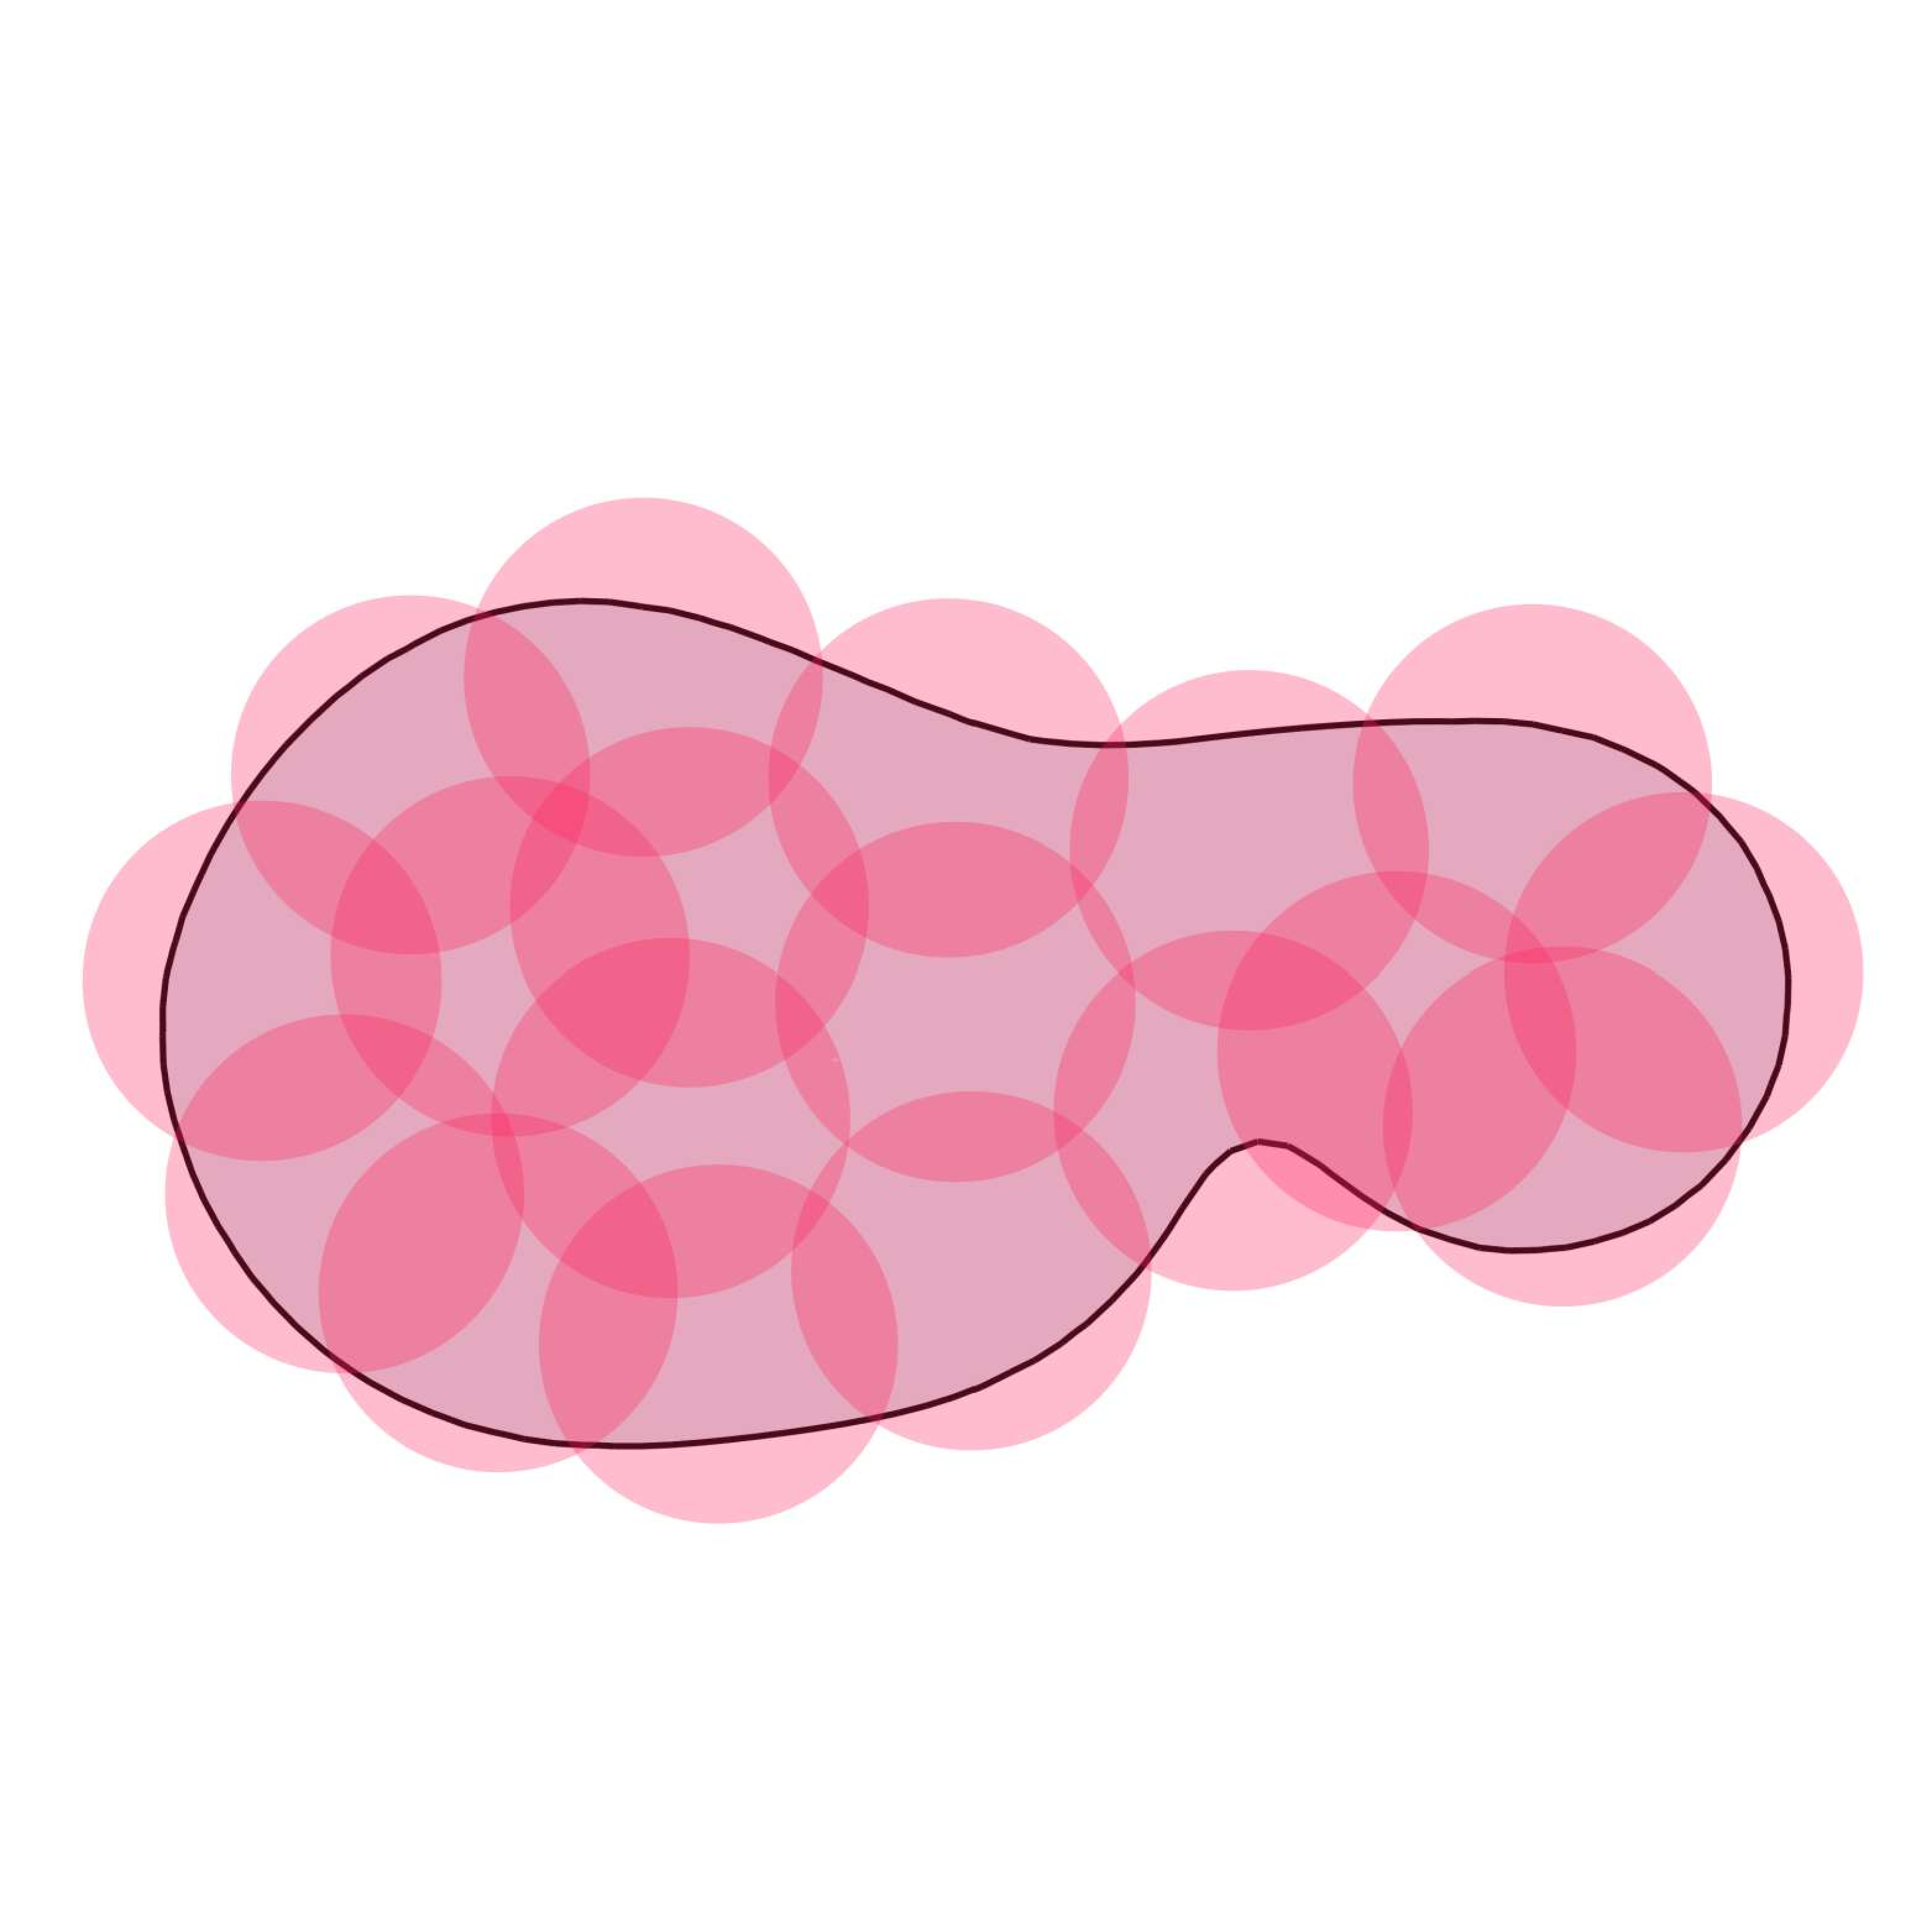
\includegraphics[trim=0 300 0 500, clip, width=0.4\textwidth]{figures/cech/cover-comp.pdf}
  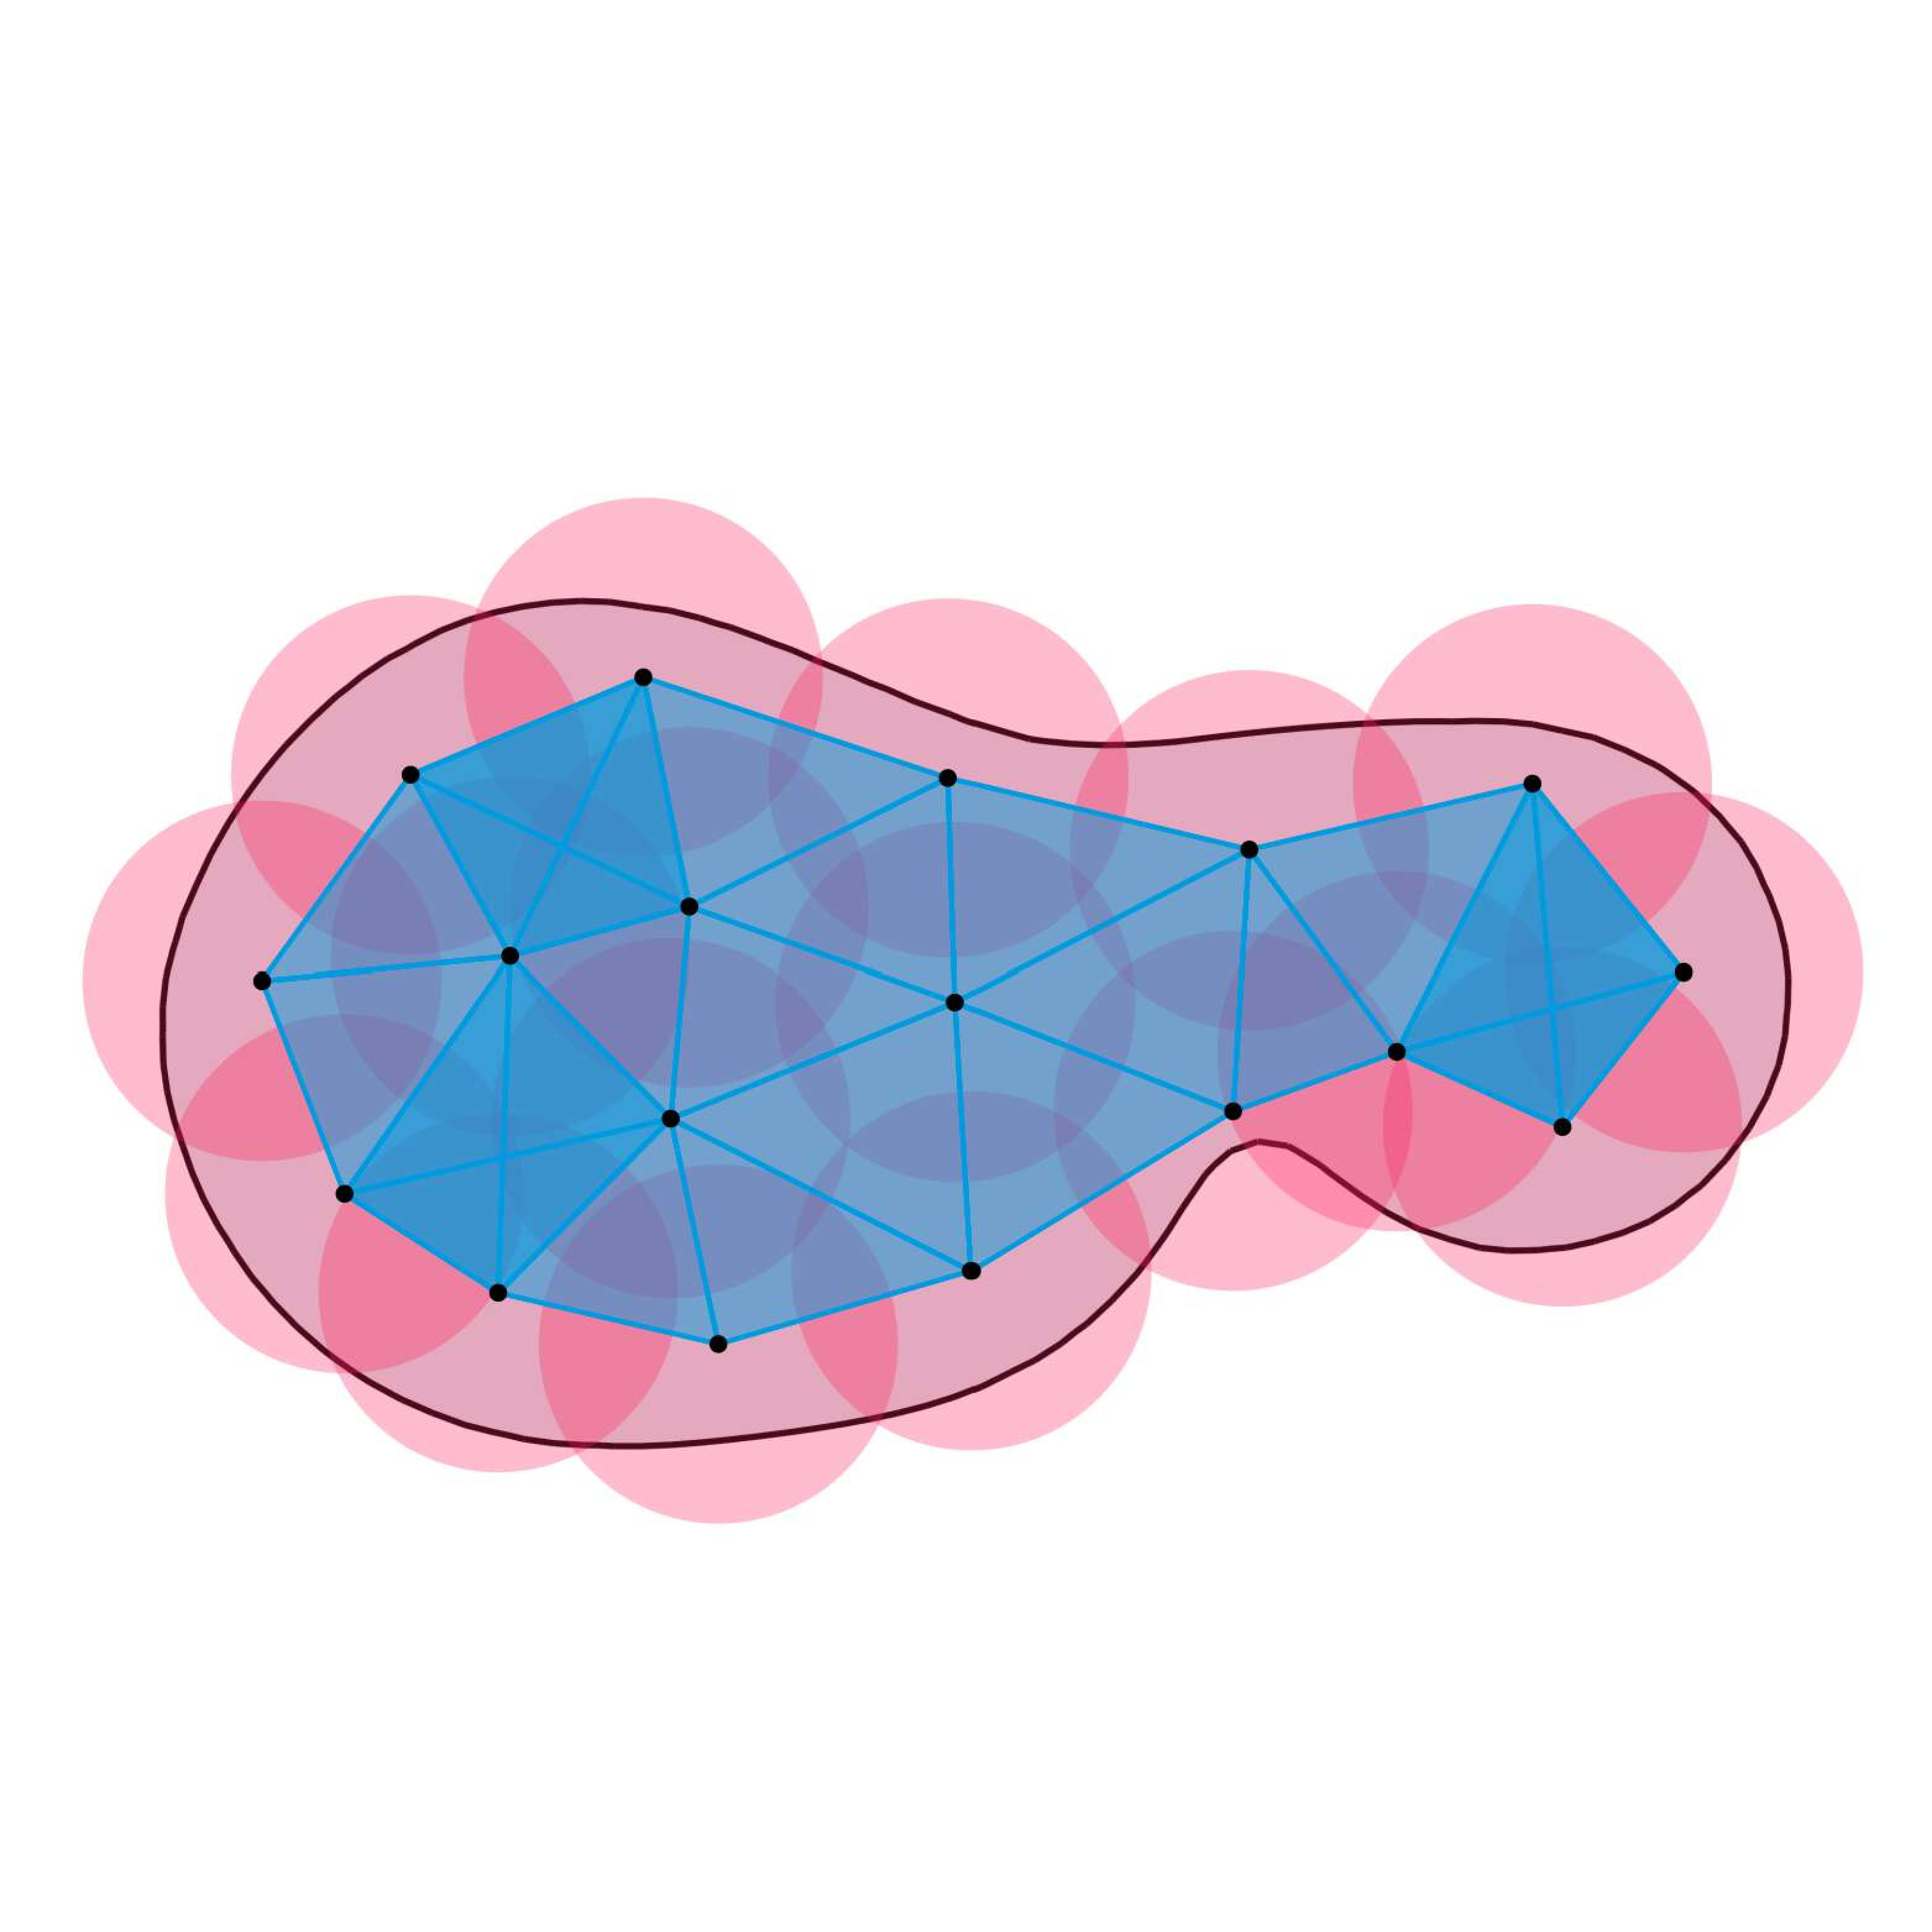
\includegraphics[trim=0 300 0 500, clip, width=0.4\textwidth]{figures/cech/full-comp.pdf}
  \caption{A metric cover and its nerve, the \v Cech complex.}\label{fig:nerves}
\end{figure}

If $(X,\dist)$ is a metric space and $P\subset X$ is a finite collection we say that $P$ covers $X$ at scale $\e$ if the collection $\U = \{\ball^\e(p)\}_{p\in P}$ is a cover of $X$.
The Nerve of this cover is known as the \textbf{\v Cech complex} at scale $\e$, denoted $\cech^\e(P)$, and is defined formally as
\[ \cech^\e(P) := \left\{\sigma \subseteq P\mid \bigcap_{p\in \sigma}\ball_\e(p)\neq \emptyset \right\}. \]
For pairs $(P, Q)$ we will write $\cech^\e(P,Q) := (\cech^\e(P), \cech^\e(Q))$ to denote the corresponding pair of \v Cech complexes.

Recalling the definition of the strong convexity radius $\varrho_X$ of a metric space $X$ we note that $\U$ is a good open cover whenever $\varrho_X > \e$.
That is, by the Nerve Theorem, the inclusion $\cech^\e(P)\hookrightarrow P^\e$ is a homotopy equivalence whenever $\varrho_X > \e$.
% The \v Cech complex provides us with a computable structure that the homotopy type of the region covered by a set of points at any scale $\varrho_X > \e$.
% Unfortunately, the \v Cech complex is difficult to compute in practice

\paragraph{The Vietoris-Rips Complex}

\begin{figure}[htbp]
  \centering
  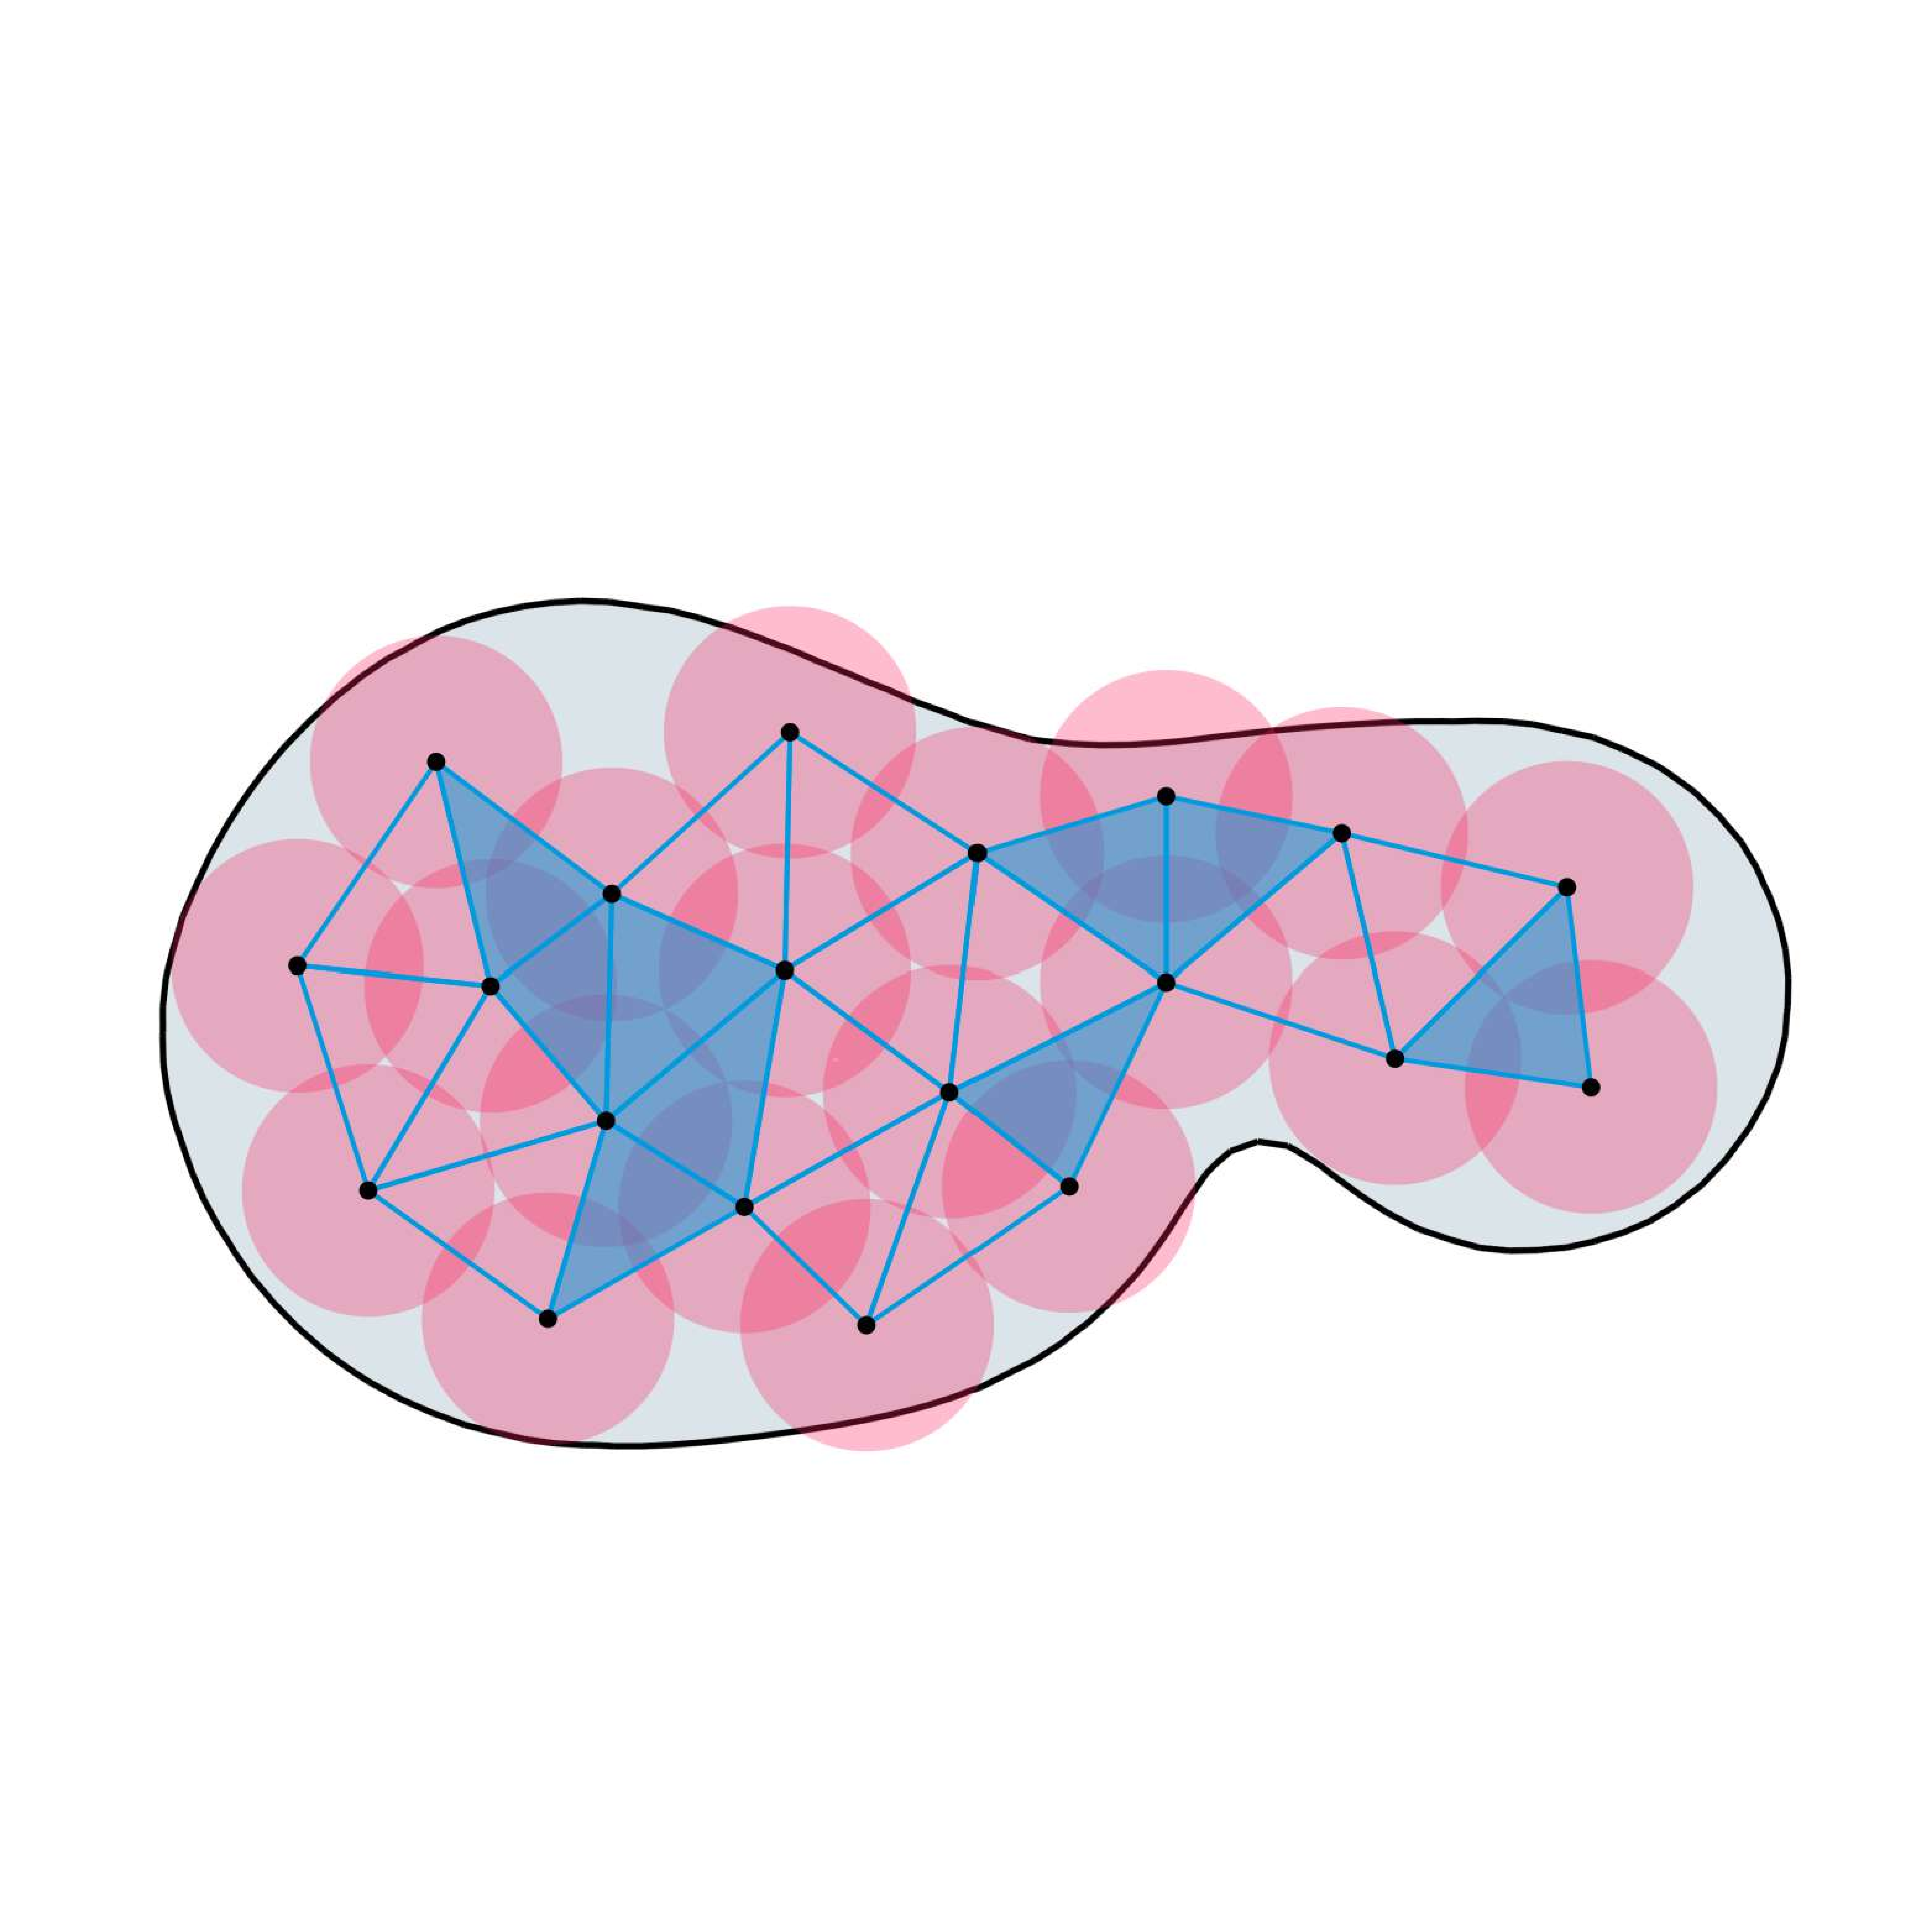
\includegraphics[trim=0 300 0 500, clip, width=0.3\textwidth]{figures/rips/cech-comp.pdf}
  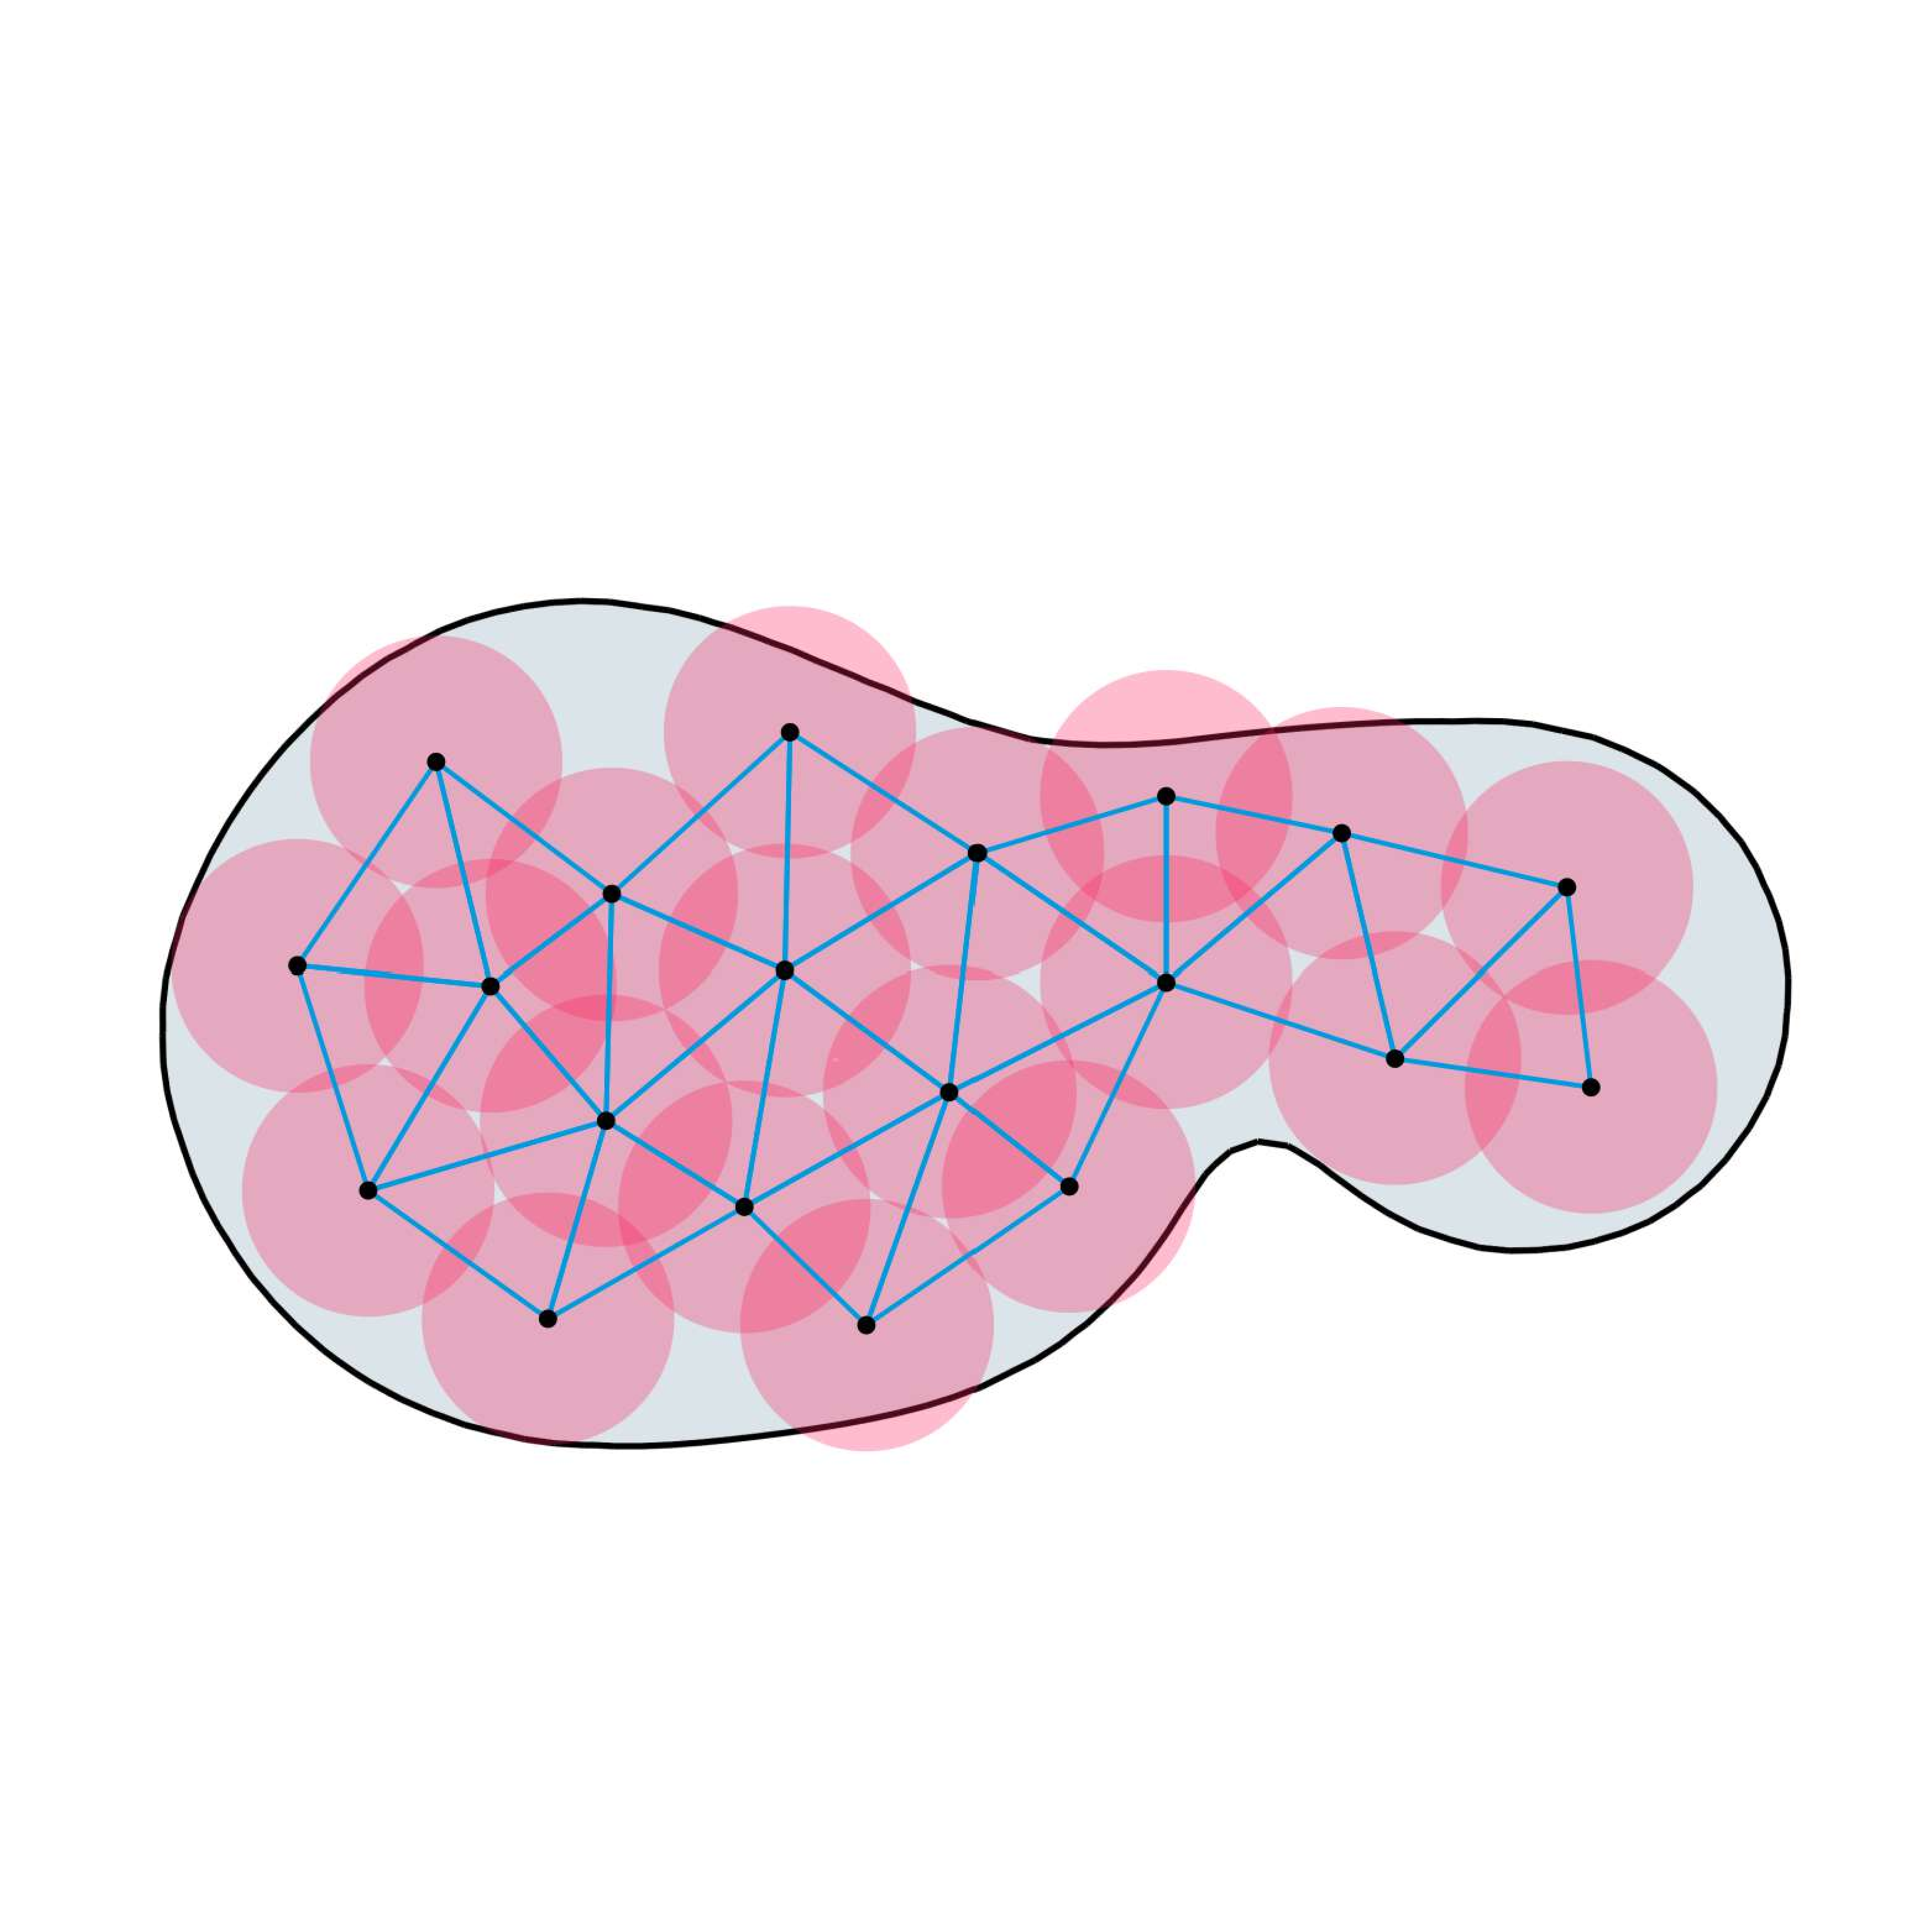
\includegraphics[trim=0 300 0 500, clip, width=0.3\textwidth]{figures/rips/graph-comp.pdf}
  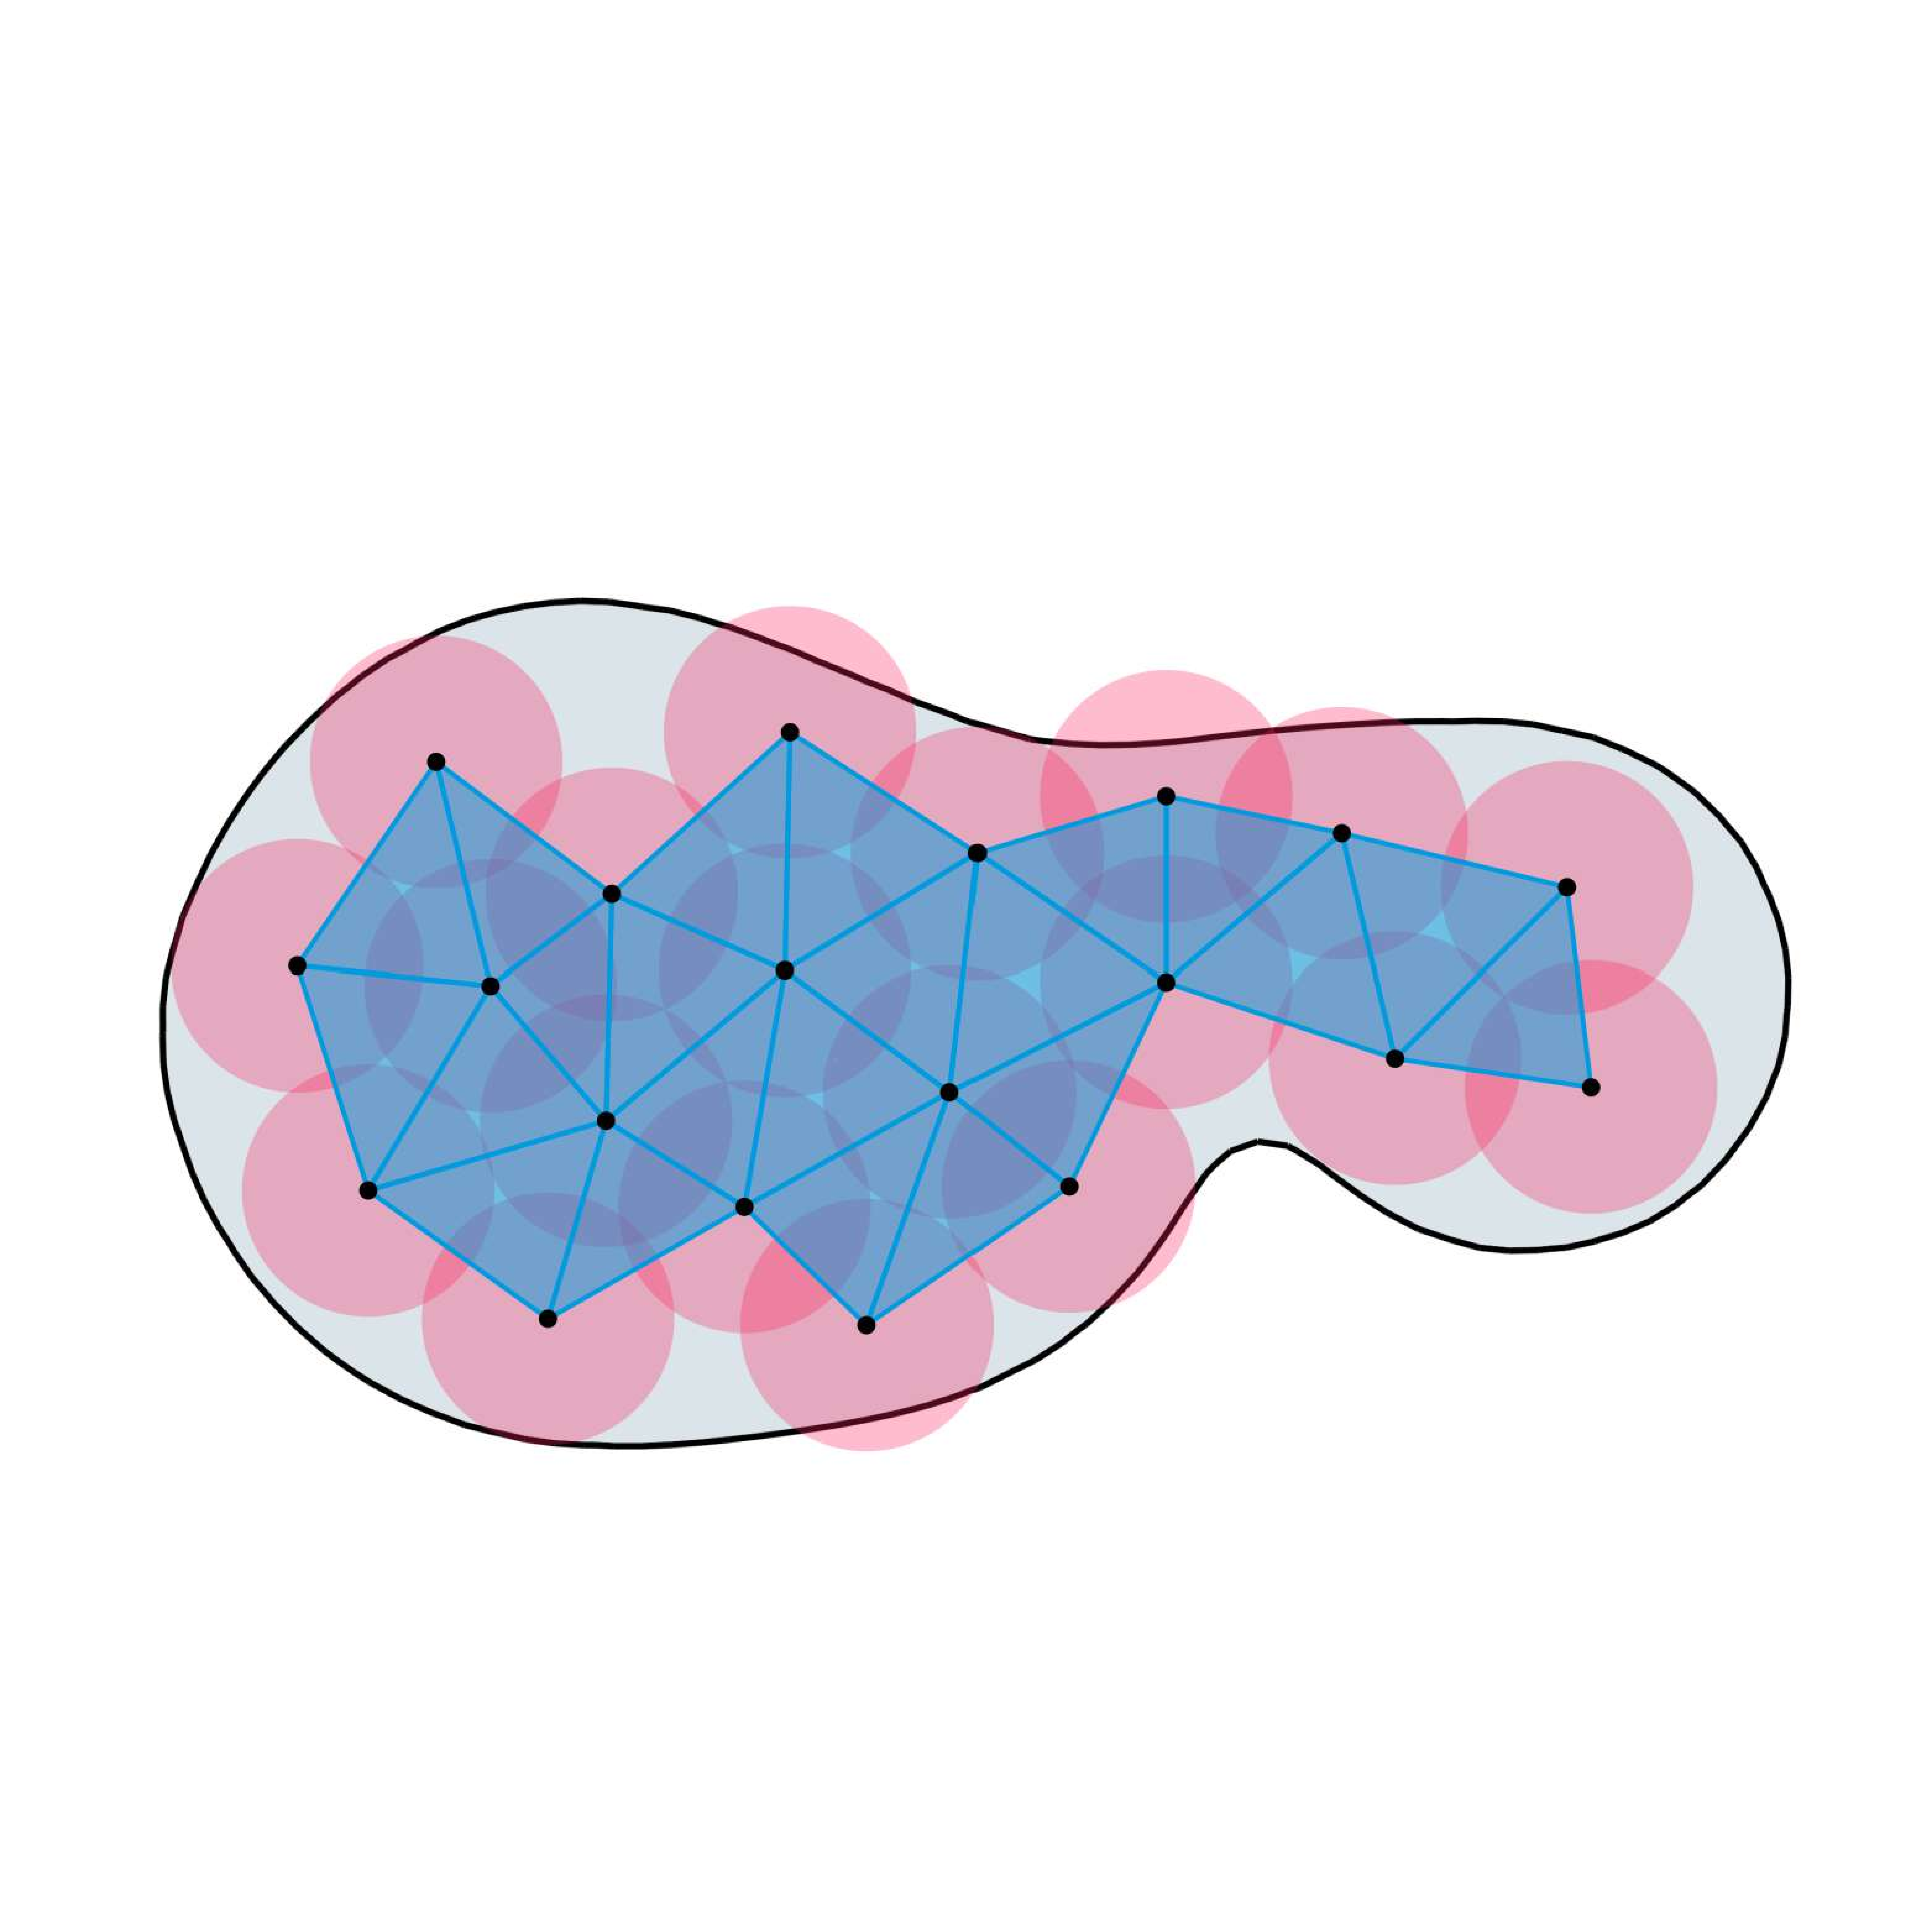
\includegraphics[trim=0 300 0 500, clip, width=0.3\textwidth]{figures/rips/rips-comp.pdf}
  \caption{The \v Cech complex $\cech^\e(P)$, $2\e$-neighborhood graph and its Clique complex, the Vietoris-Rips complex $\rips^{2\e}(P)$.}\label{fig:rips}
\end{figure}

Given an undirected graph $G = (V, E)$ we can construct a simplicial complex $K$ with vertex set $V$ and simplices $\sigma\subseteq V$ whenever $\{u,v\}\in E$ for all distinct $u, v\in\sigma$.
This is known as the \emph{clique complex} of the graph $G$.

Just as the \v Cech complex is the Nerve of metric cover sets there is a closely related simplicial complex that is the clique complex of a neighborhood graph.
That is, a graph $G$ with vertices $V$ corresponding to points in a metric space $(X,\dist)$ and $\{u,v\}\in E$ whenever $\dist(u,v)\leq \e$ for some $\e > 0$.
This is known as the \textbf{(Vietoris-)Rips complex}, and is formally defined for a finite set $P$ at scale $\e > 0$ as
\[ \rips^\e(P) = \left\{\sigma \subseteq P\mid \forall p,q\in\sigma,\ \dist(p, q)\leq \e\right\}. \]
For a pair $(P, Q)$ we will write $\rips^\e(P,Q) := (\rips^\e(P), \rips^\e(Q))$ to denote the corresponding pair of rips complexes.

By the Nerve Theorem we can use the \v Cech complex to compute the homotopy type of metric space $(X, \dist)$ covered by a finite set $P$ at any scale $\e < \varrho_X$.
Unfortunately, constructing the \v Cech complex is not feasible in practice.
We will therefore use pairs of Rips complex to capture to homotopy type of the \v Cech complex by making use of the following inclusion:
\[ \rips^\e(P) \subseteq \cech^\e(P)\subseteq \rips^{2\e}(P).\]
